% Options for packages loaded elsewhere
% Options for packages loaded elsewhere
\PassOptionsToPackage{unicode}{hyperref}
\PassOptionsToPackage{hyphens}{url}
\PassOptionsToPackage{dvipsnames,svgnames,x11names}{xcolor}
%
\documentclass[
  chinese,
]{ctexart}
\usepackage{xcolor}
\usepackage[margin=1in]{geometry}
\usepackage{amsmath,amssymb}
\setcounter{secnumdepth}{-\maxdimen} % remove section numbering
\usepackage{iftex}
\ifPDFTeX
  \usepackage[T1]{fontenc}
  \usepackage[utf8]{inputenc}
  \usepackage{textcomp} % provide euro and other symbols
\else % if luatex or xetex
  \usepackage{unicode-math} % this also loads fontspec
  \defaultfontfeatures{Scale=MatchLowercase}
  \defaultfontfeatures[\rmfamily]{Ligatures=TeX,Scale=1}
\fi
\usepackage{lmodern}
\ifPDFTeX\else
  % xetex/luatex font selection
\fi
% Use upquote if available, for straight quotes in verbatim environments
\IfFileExists{upquote.sty}{\usepackage{upquote}}{}
\IfFileExists{microtype.sty}{% use microtype if available
  \usepackage[]{microtype}
  \UseMicrotypeSet[protrusion]{basicmath} % disable protrusion for tt fonts
}{}
\makeatletter
\@ifundefined{KOMAClassName}{% if non-KOMA class
  \IfFileExists{parskip.sty}{%
    \usepackage{parskip}
  }{% else
    \setlength{\parindent}{0pt}
    \setlength{\parskip}{6pt plus 2pt minus 1pt}}
}{% if KOMA class
  \KOMAoptions{parskip=half}}
\makeatother
% Make \paragraph and \subparagraph free-standing
\makeatletter
\ifx\paragraph\undefined\else
  \let\oldparagraph\paragraph
  \renewcommand{\paragraph}{
    \@ifstar
      \xxxParagraphStar
      \xxxParagraphNoStar
  }
  \newcommand{\xxxParagraphStar}[1]{\oldparagraph*{#1}\mbox{}}
  \newcommand{\xxxParagraphNoStar}[1]{\oldparagraph{#1}\mbox{}}
\fi
\ifx\subparagraph\undefined\else
  \let\oldsubparagraph\subparagraph
  \renewcommand{\subparagraph}{
    \@ifstar
      \xxxSubParagraphStar
      \xxxSubParagraphNoStar
  }
  \newcommand{\xxxSubParagraphStar}[1]{\oldsubparagraph*{#1}\mbox{}}
  \newcommand{\xxxSubParagraphNoStar}[1]{\oldsubparagraph{#1}\mbox{}}
\fi
\makeatother


\usepackage{longtable,booktabs,array}
\newcounter{none} % for unnumbered tables
\usepackage{calc} % for calculating minipage widths
% Correct order of tables after \paragraph or \subparagraph
\usepackage{etoolbox}
\makeatletter
\patchcmd\longtable{\par}{\if@noskipsec\mbox{}\fi\par}{}{}
\makeatother
% Allow footnotes in longtable head/foot
\IfFileExists{footnotehyper.sty}{\usepackage{footnotehyper}}{\usepackage{footnote}}
\makesavenoteenv{longtable}
\usepackage{graphicx}
\makeatletter
\newsavebox\pandoc@box
\newcommand*\pandocbounded[1]{% scales image to fit in text height/width
  \sbox\pandoc@box{#1}%
  \Gscale@div\@tempa{\textheight}{\dimexpr\ht\pandoc@box+\dp\pandoc@box\relax}%
  \Gscale@div\@tempb{\linewidth}{\wd\pandoc@box}%
  \ifdim\@tempb\p@<\@tempa\p@\let\@tempa\@tempb\fi% select the smaller of both
  \ifdim\@tempa\p@<\p@\scalebox{\@tempa}{\usebox\pandoc@box}%
  \else\usebox{\pandoc@box}%
  \fi%
}
% Set default figure placement to htbp
\def\fps@figure{htbp}
\makeatother



\ifLuaTeX
\usepackage[bidi=basic,shorthands=off,provide=*]{babel}
\else
\usepackage[bidi=default,shorthands=off,provide=*]{babel}
\fi
\ifLuaTeX
  \usepackage{selnolig} % disable illegal ligatures
\fi


\setlength{\emergencystretch}{3em} % prevent overfull lines

\providecommand{\tightlist}{%
  \setlength{\itemsep}{0pt}\setlength{\parskip}{0pt}}



 


\usepackage{array}
\usepackage{booktabs}
\usepackage{longtable}
\usepackage{tabularx}
\newcolumntype{Y}{>{\raggedright\arraybackslash}X}
\usepackage{changepage}
\usepackage{xcolor}
\makeatletter
\@ifpackageloaded{caption}{}{\usepackage{caption}}
\AtBeginDocument{%
\ifdefined\contentsname
  \renewcommand*\contentsname{目录}
\else
  \newcommand\contentsname{目录}
\fi
\ifdefined\listfigurename
  \renewcommand*\listfigurename{图索引}
\else
  \newcommand\listfigurename{图索引}
\fi
\ifdefined\listtablename
  \renewcommand*\listtablename{表索引}
\else
  \newcommand\listtablename{表索引}
\fi
\ifdefined\figurename
  \renewcommand*\figurename{图}
\else
  \newcommand\figurename{图}
\fi
\ifdefined\tablename
  \renewcommand*\tablename{表}
\else
  \newcommand\tablename{表}
\fi
}
\@ifpackageloaded{float}{}{\usepackage{float}}
\floatstyle{ruled}
\@ifundefined{c@chapter}{\newfloat{codelisting}{h}{lop}}{\newfloat{codelisting}{h}{lop}[chapter]}
\floatname{codelisting}{列表}
\newcommand*\listoflistings{\listof{codelisting}{列表索引}}
\makeatother
\makeatletter
\makeatother
\makeatletter
\@ifpackageloaded{caption}{}{\usepackage{caption}}
\@ifpackageloaded{subcaption}{}{\usepackage{subcaption}}
\makeatother
\usepackage{bookmark}
\IfFileExists{xurl.sty}{\usepackage{xurl}}{} % add URL line breaks if available
\urlstyle{same}
% fallback for those not using the hyperref driver hyperxmp:
\makeatletter
\@ifundefined{xmpquote}{\newcommand{\xmpquote}[1]{#1}}{}
\makeatother
\hypersetup{
  pdftitle={第13讲 VLA 前沿：跑得更快、记得更久、用上全身},
  pdflang={zh-CN},
  colorlinks=true,
  linkcolor={blue},
  filecolor={Maroon},
  citecolor={Blue},
  urlcolor={Blue},
  pdfcreator={LaTeX via pandoc}}


\title{第13讲 VLA 前沿：跑得更快、记得更久、用上全身}
\author{}
\date{}
\begin{document}
\maketitle

\renewcommand*\contentsname{目录}
{
\setcounter{tocdepth}{3}
\tableofcontents
}

上一讲我们把一个 VLA
微调到了自己的机器人上，让它在桌面任务里能跑、能用。这一讲往前看：把一个能用的
VLA
推向真实落地，会立刻撞上三道前沿难题------它\textbf{太慢}，跟不上控制频率；它\textbf{记不住}，长程任务做着做着就乱；它\textbf{只有一只手}，没法用整个人形身体去干活。

这三道题各自都已经长出一条活跃的研究线。本讲不展开任何一篇的全部细节，而是沿三个方向各画一张路线地图、各挑几篇代表作把直觉讲透：实时推理让
VLA 跑得更快，长时记忆让它记得更久，人形全身 VLA
让它用上整个身体。这是一讲前沿综述，不配实验；目标是让你建立''VLA
接下来往哪走''的全局判断。

\section{1
实时推理：让大模型跟上控制频率}\label{ux5b9eux65f6ux63a8ux7406ux8ba9ux5927ux6a21ux578bux8ddfux4e0aux63a7ux5236ux9891ux7387}

\subsection{1.1 为什么''实时''是 VLA
落地的第一个卡点}\label{ux4e3aux4ec0ux4e48ux5b9eux65f6ux662f-vla-ux843dux5730ux7684ux7b2cux4e00ux4e2aux5361ux70b9}

当前主流大 VLA 推理一次------图像编码 + 语言模型 prefill +
动作去噪------完整跑一轮往往要 58--106
ms，还不含网络通信。这个数字本身不算''慢''，要判断它够不够快，得放到机器人自己的时间预算里去比：

\begin{center}
\begin{tabular}{@{}>{\raggedright\arraybackslash}p{\dimexpr 0.2226\linewidth - 2\tabcolsep\relax} >{\raggedright\arraybackslash}p{\dimexpr 0.7774\linewidth - 2\tabcolsep\relax}@{}}
\toprule\noalign{}
指标 & 含义 \\
\midrule\noalign{}
首动作延迟 & 从拿到新观测，到第一个可执行动作发出去，隔了多久 \\
感知到动作端到端延迟 & 传感器采样 → 预处理 → 推理 → 后处理 → 下发的全链路耗时 \\
闭环重规划周期 & 多久重新看一眼环境、重新规划一次 \\
动作块边界停顿 & 一个块执行完、下一个块还没算好时，机器人空等多久 \\
任务允许时限 & 这个任务留给你的机会窗口有多长（抓传送带上的物体 vs 慢速摆放，差好几个数量级） \\
\bottomrule\noalign{}
\end{tabular}
\end{center}

拿这套口径去量，问题就具体了：

\begin{itemize}
\tightlist
\item
  \textbf{停顿}：推理还没算完，机器人只能等，在动作块边界出现可见停顿，动态任务直接失败。
\item
  \textbf{抖动}：相邻两次规划可能选不同路径，切换点剧烈震动，触发保护停机。
\item
  \textbf{反应盲区}：就算消除了停顿，感知到新信息后仍要等整个推理流程跑完才能给出第一个动作------几十毫秒的首动作延迟，在乒乓球、传送带分拣这类任务里足以让机会窗口关闭。
\end{itemize}

一句话：\textbf{大 VLA
单次推理几十到上百毫秒，而真实控制要高频、低延迟、快反应。}
这不是调参能抹平的矛盾，需要从算法、系统、学习三个层面协同突破。

\begin{quote}
备注：常见的一种类比是''人的反应时间约 150--200 ms，所以模型 58--106 ms
已经够快（或还不够快）``。这个对比其实不成立：人的反应时间包含感知、决策与肌肉启动的完整链路，而
VLA
那个数字只是推理这一段，两者不是同一个指标，不能直接比大小。要谈够不够快，就用上表这些机器人侧的量。
\end{quote}

\subsection{1.2 三条路线：算法 / 系统 /
学习+投机}\label{ux4e09ux6761ux8defux7ebfux7b97ux6cd5-ux7cfbux7edf-ux5b66ux4e60ux6295ux673a}

同一个''实时''目标，有三种正交的解法。先把地图立起来：

\begin{center}
\begin{tabular}{@{}>{\raggedright\arraybackslash}p{\dimexpr 0.0951\linewidth - 2\tabcolsep\relax} >{\raggedright\arraybackslash}p{\dimexpr 0.3681\linewidth - 2\tabcolsep\relax} >{\raggedright\arraybackslash}p{\dimexpr 0.2572\linewidth - 2\tabcolsep\relax} >{\raggedright\arraybackslash}p{\dimexpr 0.2796\linewidth - 2\tabcolsep\relax}@{}}
\toprule\noalign{}
路线 & 关键问题 & 代表工作 & 核心手段 \\
\midrule\noalign{}
\textbf{算法层} & 推理没算完怎么执行不停顿、不抖动？感知到变化怎么快速反应？ & RTC、FASTER & 改推理期调度策略；不改模型、不改训练 \\
\textbf{系统层} & 模型本身太慢，怎么进 30 ms 以内？ & Realtime-VLA V1 & kernel 工程 + 并发流水线，榨干硬件 \\
\textbf{学习+投机层} & 跑快了不稳不准怎么办？重复规划能否少推理几次？ & Realtime-VLA V2、Flash & 学习速度自适应；投机推理跳过昂贵去噪 \\
\bottomrule\noalign{}
\end{tabular}
\end{center}

三条路线互补而非竞争：算法层免训练、即插即用；系统层是底层使能，没有它的速度基础，上面两层都无从谈起；学习+投机层在''已经快''的基础上，把平均延迟进一步压到极限。下面挑三篇把直觉讲透。

\subsection{1.3
RTC：把''等推理''变成''边算边接''}\label{rtcux628aux7b49ux63a8ux7406ux53d8ux6210ux8fb9ux7b97ux8fb9ux63a5}

第一道坎是停顿与抖动。以 \(\pi_{0.5}\) 为例：一次\textbf{模型推理}要 76
ms，而底层控制器每 20 ms 就要消费一个动作（即\textbf{动作执行周期} 20
ms，不是每 20 ms 重新推理一次）。动作队列能按 20 ms
稳定出队，靠的是一次推理生成了一整块动作；可一旦这一块执行到底、下一块还没算出来，``算完再动''就意味着每个动作块边界都卡顿。更糟的是相邻两块可能各走各的路，切换点直接抖到触发保护停机。

\begin{figure}[H]

{\centering 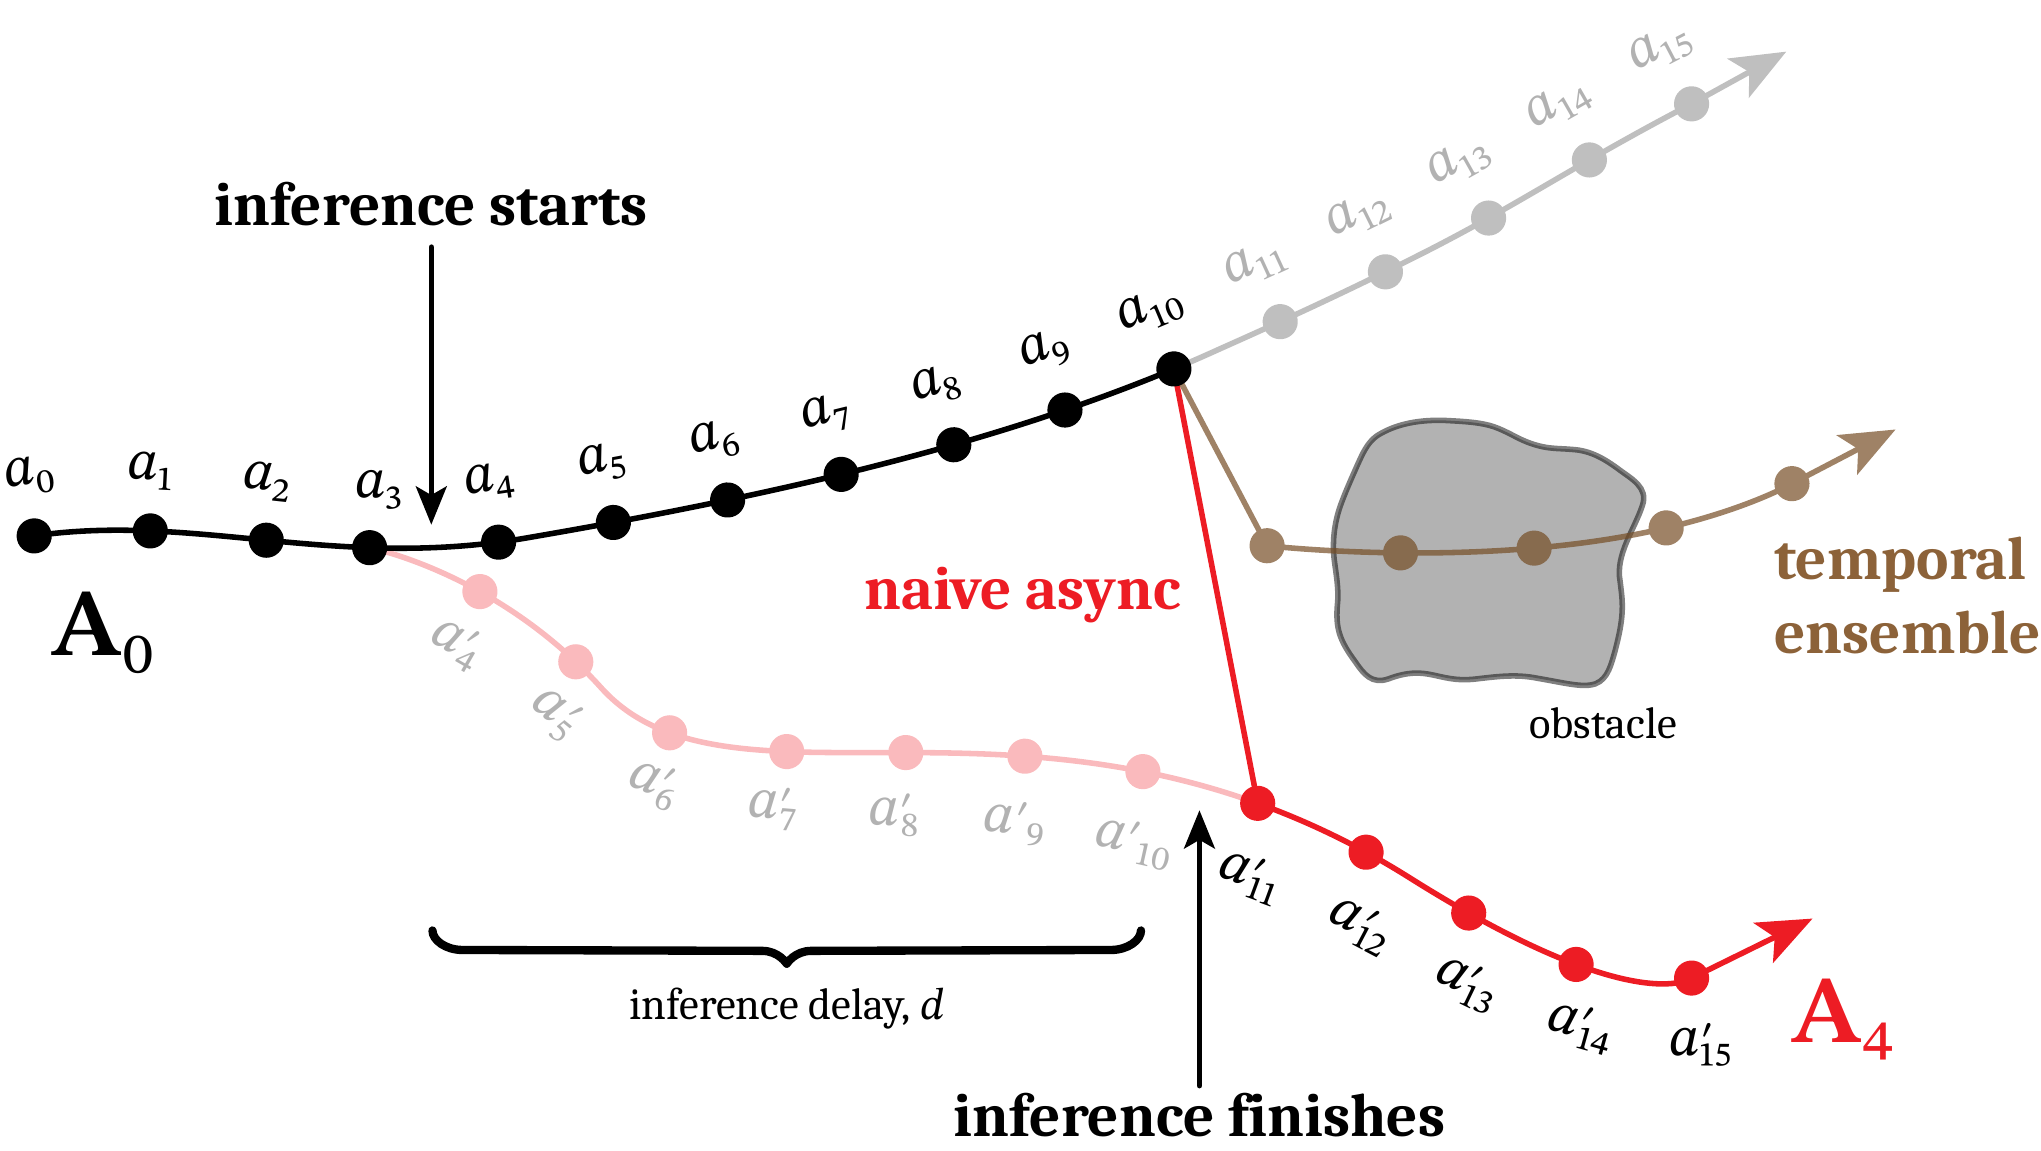
\includegraphics[width=0.68\linewidth,height=\textheight,keepaspectratio]{../../assets/figures/lecture13/ref/rt_rtc_bifurcation.png}

}

\caption{朴素异步在切换点猛地一跳，取平均又会穿过障碍物------两种简单做法都不行}

\end{figure}%

RTC{[}1{]}
的做法可以类比成\textbf{修图}：已经在执行、来不及改的动作直接''冻住''，只对还没到的未来段重新生成，接缝处用软过渡保证连续。

\begin{figure}[H]

{\centering 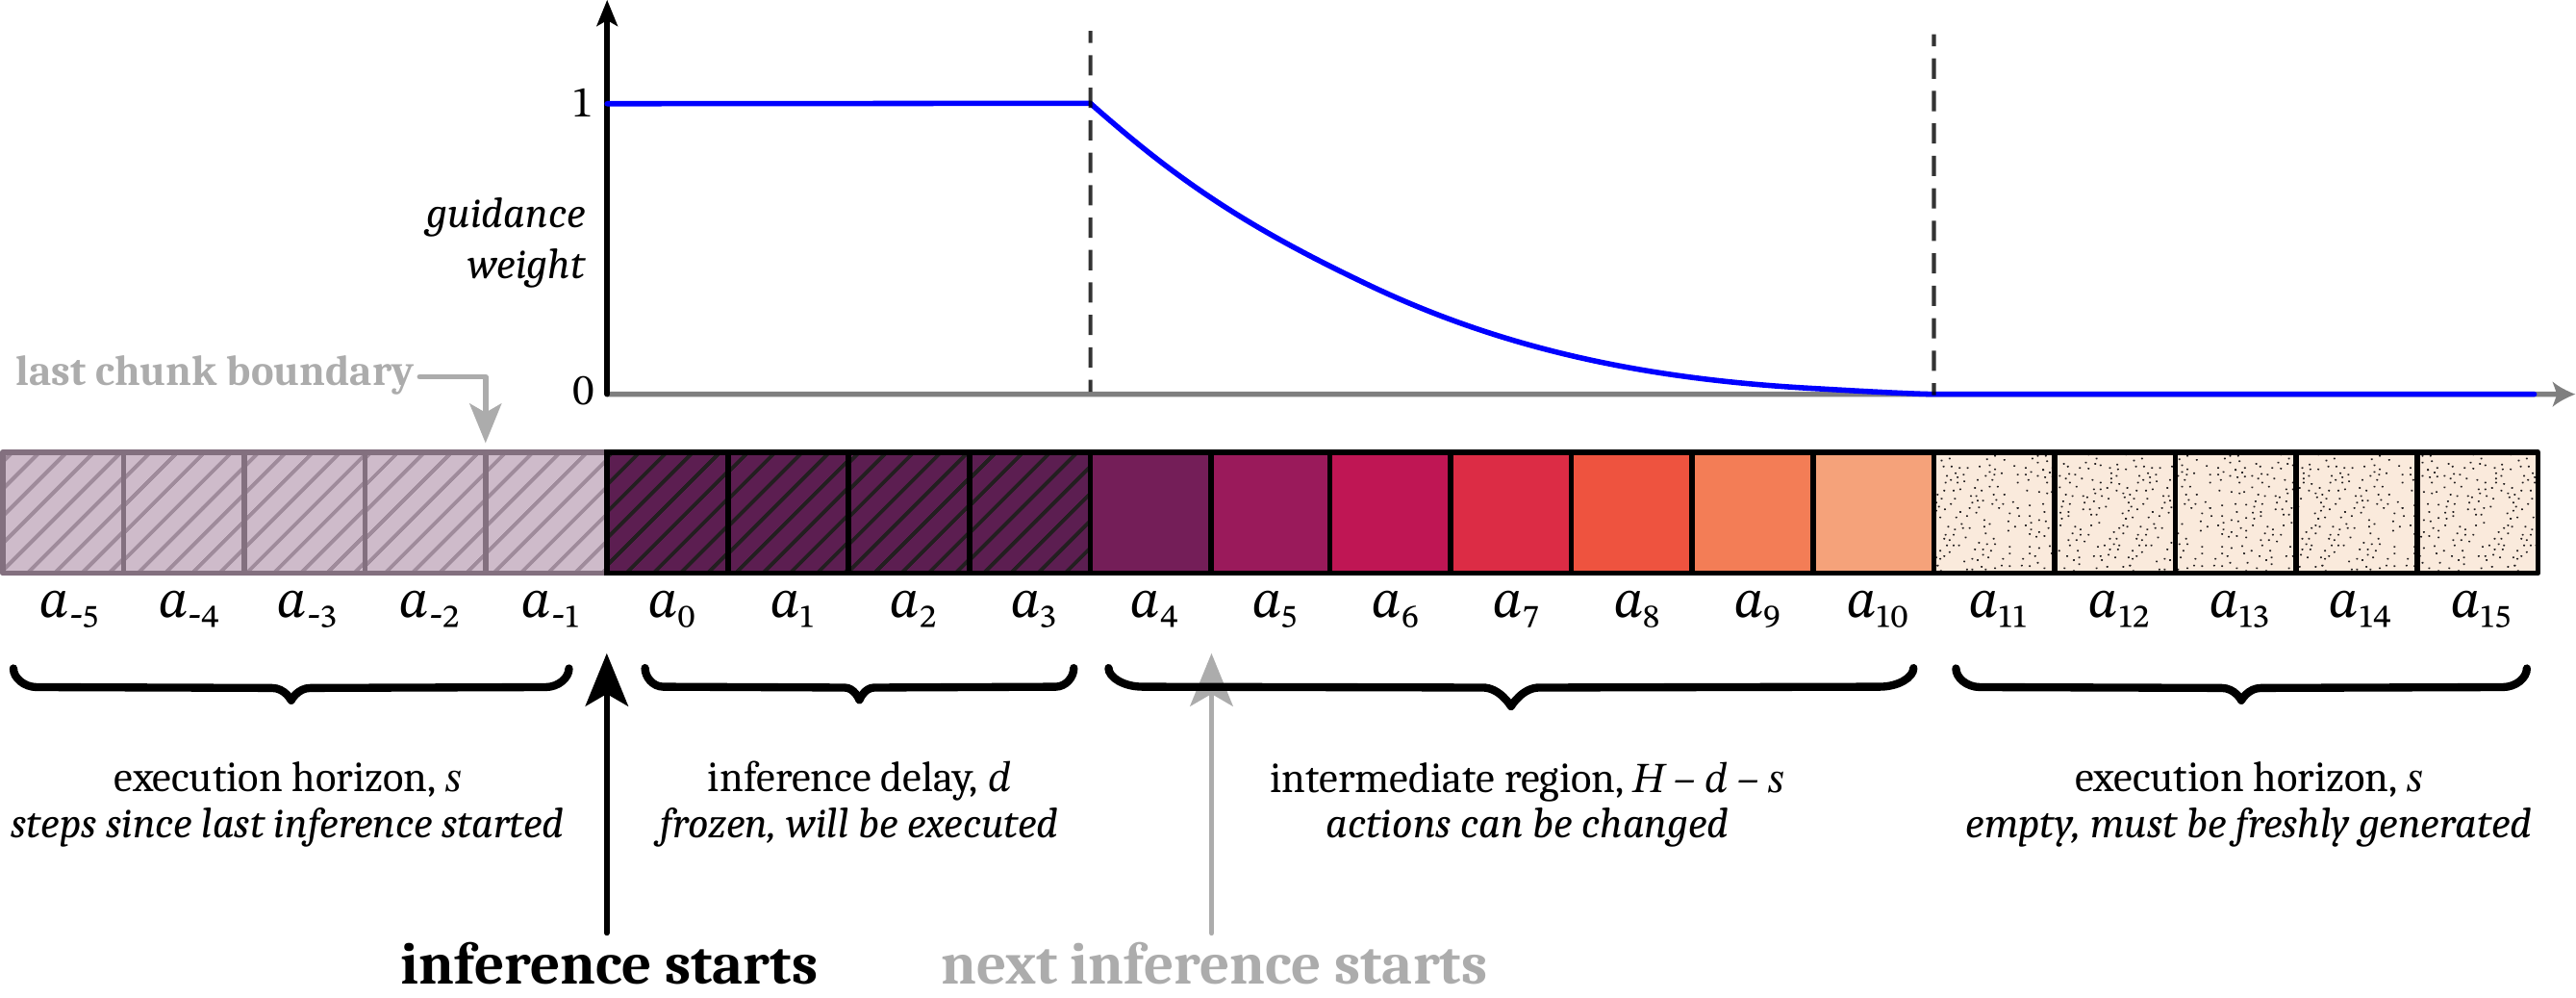
\includegraphics[width=0.8\linewidth,height=\textheight,keepaspectratio]{../../assets/figures/lecture13/ref/rt_rtc_diagram.png}

}

\caption{把一个动作块切成''冻结 / 软过渡 /
自由重画''三段，只重画未来段，接缝平滑}

\end{figure}%

它完全免训练、即插即用，在注入 +100 / +200 ms
延迟时依然不崩。它解决的是''一个块怎么平滑地接到下一个块''。

\subsection{1.4
FASTER：不只不卡，还要反应快}\label{fasterux4e0dux53eaux4e0dux5361ux8fd8ux8981ux53cdux5e94ux5feb}

执行平滑了还不够。打乒乓球这种任务，球飞过来到要挥拍只有几百毫秒------机器人''看到''之后还得等整轮去噪（比如
10 步）跑完才出第一个动作，机会窗口早就关了。

\begin{figure}[H]

{\centering 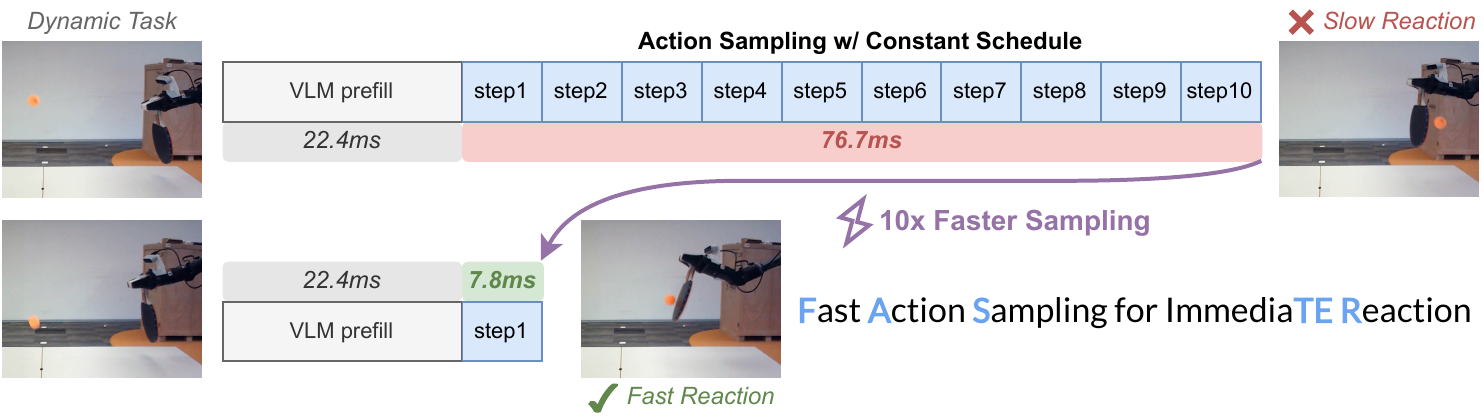
\includegraphics[width=0.86\linewidth,height=\textheight,keepaspectratio]{../../assets/figures/lecture13/ref/rt_faster_teaser.png}

}

\caption{恒定调度要等 76.7 ms 才出第一个动作，FASTER 把它压到 7.8 ms}

\end{figure}%

FASTER{[}2{]}
的关键观察是：近端动作路径直，\textbf{一步就能估准}，只有远端动作才真正需要多步去噪。于是让近端动作一算好就立刻发给机器人，不必等整块凑齐。

\begin{figure}[H]

{\centering 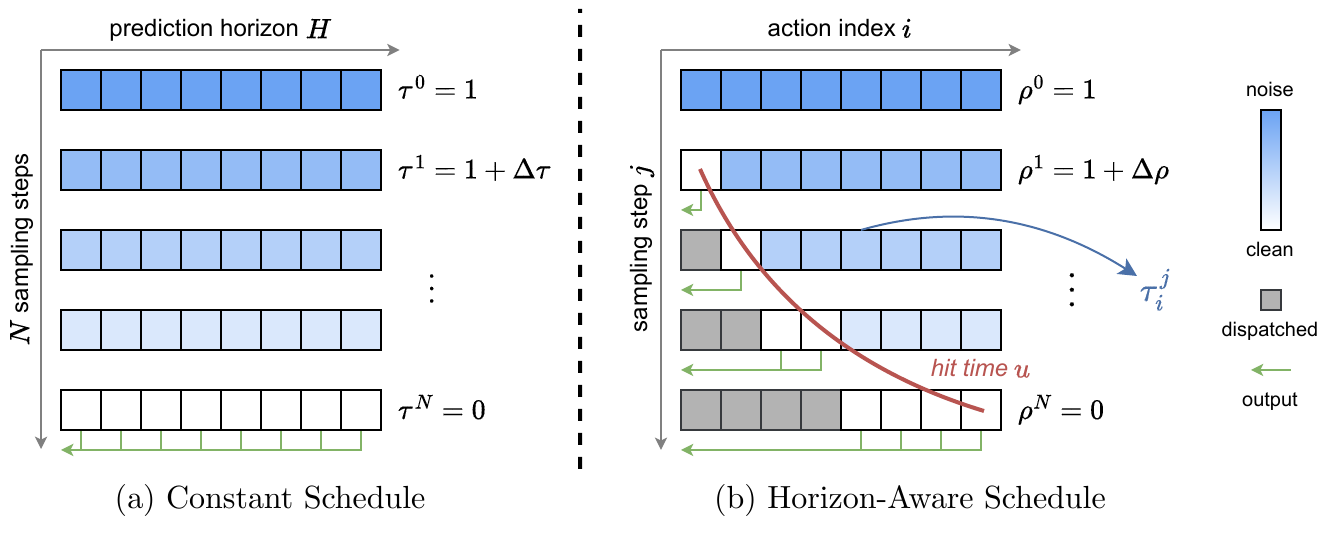
\includegraphics[width=0.8\linewidth,height=\textheight,keepaspectratio]{../../assets/figures/lecture13/ref/rt_faster_schedule.png}

}

\caption{恒定调度 vs Horizon-Aware 调度：近端动作提前完成、提前发出}

\end{figure}%

反应速度（出第一个动作的时间）约 \textbf{10× 加速}。RTC 和 FASTER
都属算法层------只改推理期的调度策略，不动模型、不重训。

\subsection{1.5 Realtime-VLA V1：把模型本身榨到 30
FPS}\label{realtime-vla-v1ux628aux6a21ux578bux672cux8eabux69a8ux5230-30-fps}

上面算法层那些做法，都是在''单次推理耗时给定''的前提下把停顿和抖动藏起来；它们没有让模型本身变快。可现实是一个
3B 的 \(\pi_0\) 用朴素 PyTorch 单次推理要 106 ms，连 30 FPS（\(\leq 33\)
ms）的重规划节奏都摸不到。这时要换一个层面：不改算法，把模型本身在硬件上跑快。

Realtime-VLA V1{[}3{]} 的核心是 \textbf{Full Streaming Inference}
框架：把''看场景''的大模型（计算密集）和''出动作''的 Action
Expert（访存密集）拆成两条频率不同的回路\textbf{并发}跑------大模型慢回路几十毫秒看一次场景，Action
Expert 快回路最快约 2 ms 就出一次动作，互不阻塞。

\begin{figure}[H]

{\centering 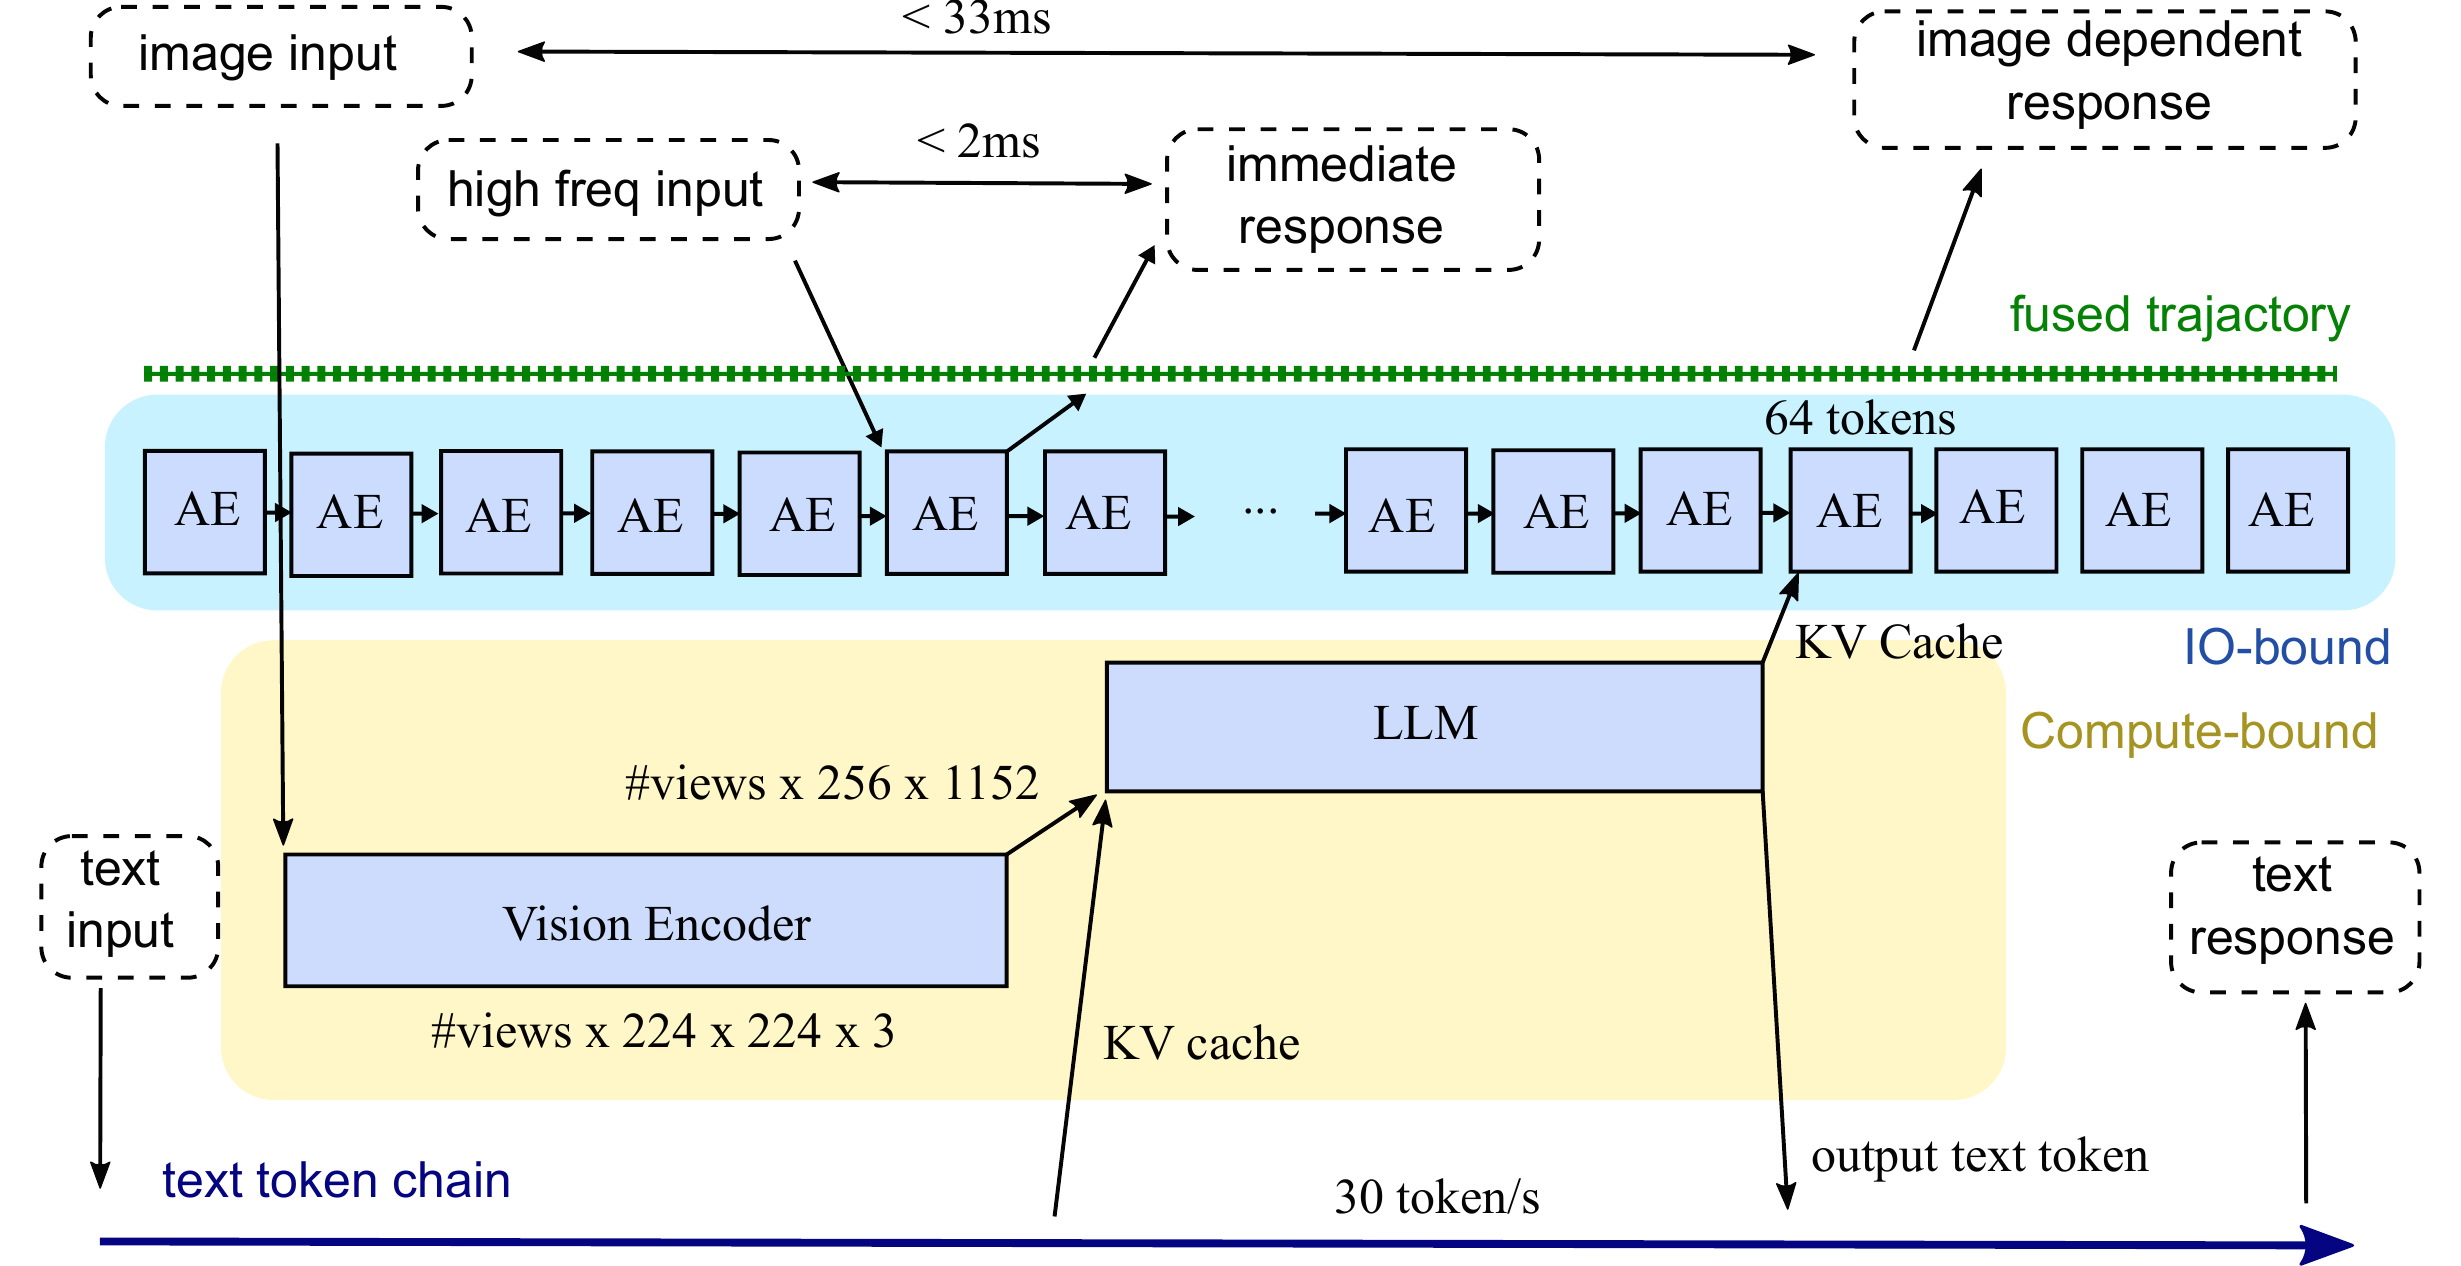
\includegraphics[width=0.82\linewidth,height=\textheight,keepaspectratio]{../../assets/figures/lecture13/ref/rt_v1_framework.png}

}

\caption{Full Streaming Inference：大模型慢回路看场景、Action Expert
快回路出轨迹，并发跑出三层不同频率}

\end{figure}%

配合 kernel 工程（把网络约化成约 24 个算子逐个手调：RMSNorm 折叠、QKV
融合等），单张 RTX 4090 双视角推理压到 \textbf{27 ms（约 37 FPS）}；再靠
Full Streaming Inference 把 Action Expert
解耦出来单独高频跑，\textbf{轨迹参考的更新频率}最高冲到 \textbf{480
Hz}。要注意这是动作专家输出轨迹参考的频率，\textbf{不等于力矩环或阻抗控制环的频率}------能不能真正满足力控
/
阻抗控制的要求，还取决于力传感、总线周期、实时操作系统、控制器稳定性与抖动，需要由底层实时控制栈单独验证。这一步也为''把高频力
/ 触觉信号训进模型''埋下伏笔------这正是 V2 要接的。

\subsection{1.6 学会调速与少推理：V2 与
Flash}\label{ux5b66ux4f1aux8c03ux901fux4e0eux5c11ux63a8ux7406v2-ux4e0e-flash}

把模型跑快之后，还有两类问题，分别由学习层和投机层来补，这里各给一句直觉：

\begin{itemize}
\tightlist
\item
  \textbf{Realtime-VLA
  V2{[}4{]}}：跑快了立刻露馅------轻量臂高速会抖、示教数据全是''舒适速度''导致一加速模型就懵。问题本质不是''能不能快''，而是\textbf{何时快、何时慢}，这得学。V2
  给出一套全栈流程（速度自适应模型定节奏 +
  时域/空域优化抹平滞后），并先把相机曝光、读出、关节反馈、运动滞后加起来近
  300 ms 的系统时延标定对齐。折衬衫、0.2 mm
  精度装配等任务能做到接近人类操作速度，精细阶段自动减速。
\item
  \textbf{Realtime-VLA
  Flash{[}5{]}}：传送带分拣里大多数时候动作和上一轮几乎一样，何必每次从头算？Flash
  借用大模型的\textbf{投机推理}：用一个便宜的小模型（约主模型的
  4\%）一步猜出整块动作（\textless8
  ms），主模型只做快速并行验证，猜对直接用，猜错或要精细抓取时才回退完整推理（\textgreater50
  ms）。任务级平均延迟降到 19 ms（约 3× 加速）。
\end{itemize}

\subsection{1.7 本节小结}\label{ux672cux8282ux5c0fux7ed3}

实时不是单点
trick，而是三条线合力：算法层（调度）消除停顿/抖动、压缩反应盲区；系统层（硬件榨取）让模型本身进
30 ms，是上层方案的速度地基；学习+投机层（自适应 +
投机）把平均延迟压到极限。缺哪一条，都只是部分答案。

\section{2 长时记忆：让 VLA
记得住、想得到}\label{ux957fux65f6ux8bb0ux5fc6ux8ba9-vla-ux8bb0ux5f97ux4f4fux60f3ux5f97ux5230}

\subsection{2.1 单帧 VLA
的马尔可夫假设为什么不够}\label{ux5355ux5e27-vla-ux7684ux9a6cux5c14ux53efux592bux5047ux8bbeux4e3aux4ec0ux4e48ux4e0dux591f}

绝大多数
VLA（OpenVLA、\(\pi_0\)、ACT\ldots\ldots）都有一个隐含假设：\textbf{当前这一帧，足以决定下一步动作}------也就是把单帧观测当成了充分统计量。

可真实操作任务常常是\textbf{部分可观测}的：单帧不足以恢复出决策所需的状态。

\begin{itemize}
\tightlist
\item
  机械臂挡住了关键区域，当前帧看不全；
\item
  ``按按钮''任务，按前按后画面几乎一样，分不清按过没有（两个不同的真实状态映射到几乎相同的观测，这叫\textbf{状态别名}）；
\item
  多阶段任务里，早一步的决定影响晚一步该怎么走；
\item
  传送带上的物体在动，得预判它会移到哪。
\end{itemize}

要说准确的话：\textbf{环境的状态转移本身可以仍是马尔可夫的}，问题出在策略只拿到了部分观测------这类问题的标准刻画是
POMDP（部分可观测马尔可夫决策过程）。所以补救办法不是''放弃马尔可夫性''，而是把决策依据从单帧扩成足以近似状态的东西：引入历史、记忆，或做状态估计。

一句话：\textbf{只看当下一帧的
VLA，既不会用过去，也不会预判未来，于是长程任务做不下来。}
这条研究线就是在回答------怎么给 VLA 装上''记忆''和''想象''。

\subsection{2.2
一条主线：从隐式上下文到记忆+想象}\label{ux4e00ux6761ux4e3bux7ebfux4eceux9690ux5f0fux4e0aux4e0bux6587ux5230ux8bb0ux5fc6ux60f3ux8c61}

这个方向的工作可以排成一条由隐到显、再从记忆走向想象的主线：

\begin{center}
\begin{tabular}{@{}>{\raggedright\arraybackslash}p{\dimexpr 0.1697\linewidth - 2\tabcolsep\relax} >{\raggedright\arraybackslash}p{\dimexpr 0.2282\linewidth - 2\tabcolsep\relax} >{\raggedright\arraybackslash}p{\dimexpr 0.6021\linewidth - 2\tabcolsep\relax}@{}}
\toprule\noalign{}
阶段 & 代表工作 & 一句话定位 \\
\midrule\noalign{}
看过去 1： 隐式 & Long-Context DP & 把历史当长上下文，用''也预测过去''正则 + 缓存训练，又好又省 \\
看过去 2： 轻量 & HAMLET & 给现成 VLA 外挂可学习 token + 轻记忆，免重训变 history-aware \\
看过去 3： 检索 & Chameleon & 观测-动作延迟；记忆要可区分 / 可寻址 / 可前瞻 \\
看过去 4： 记忆库 & MemoryVLA & 仿海马体的显式感知-认知记忆库：检索-融合-巩固 \\
看过去 5： 双记忆 & Dual-Memory VLA & 把''先验''和''近期动作一致性''也当记忆，生成又快又稳 \\
看未来 1： 想象 & MemoryVLA++ & 在记忆之上加世界模型，潜空间想象未来 \\
看未来 2： 预测 & BagelVLA & 语言规划 + 视觉预测 + 动作交错统一，单步残差低延迟 \\
长程收口 & Long-VLA & 输入掩码把子任务切成移动 / 交互两段，端到端拿到技能串接 \\
\bottomrule\noalign{}
\end{tabular}
\end{center}

前五行在''用好过去''，第六七行加上''预判未来''，最后一行直指''长程''。下面挑三篇把这条线讲透，先点一个判别标尺。

\subsection{2.3 记忆要''找得回、用得上''：Chameleon
的三条标尺}\label{ux8bb0ux5fc6ux8981ux627eux5f97ux56deux7528ux5f97ux4e0achameleon-ux7684ux4e09ux6761ux6807ux5c3a}

Chameleon{[}6{]}
用\textbf{猜杯子}点破问题：先看到球藏在哪个杯子下、洗牌后球已不可见、最后却要选对------决定动作的信息早被看到、用时却已看不见，这叫\textbf{观测-动作延迟}。

\begin{figure}[H]

{\centering 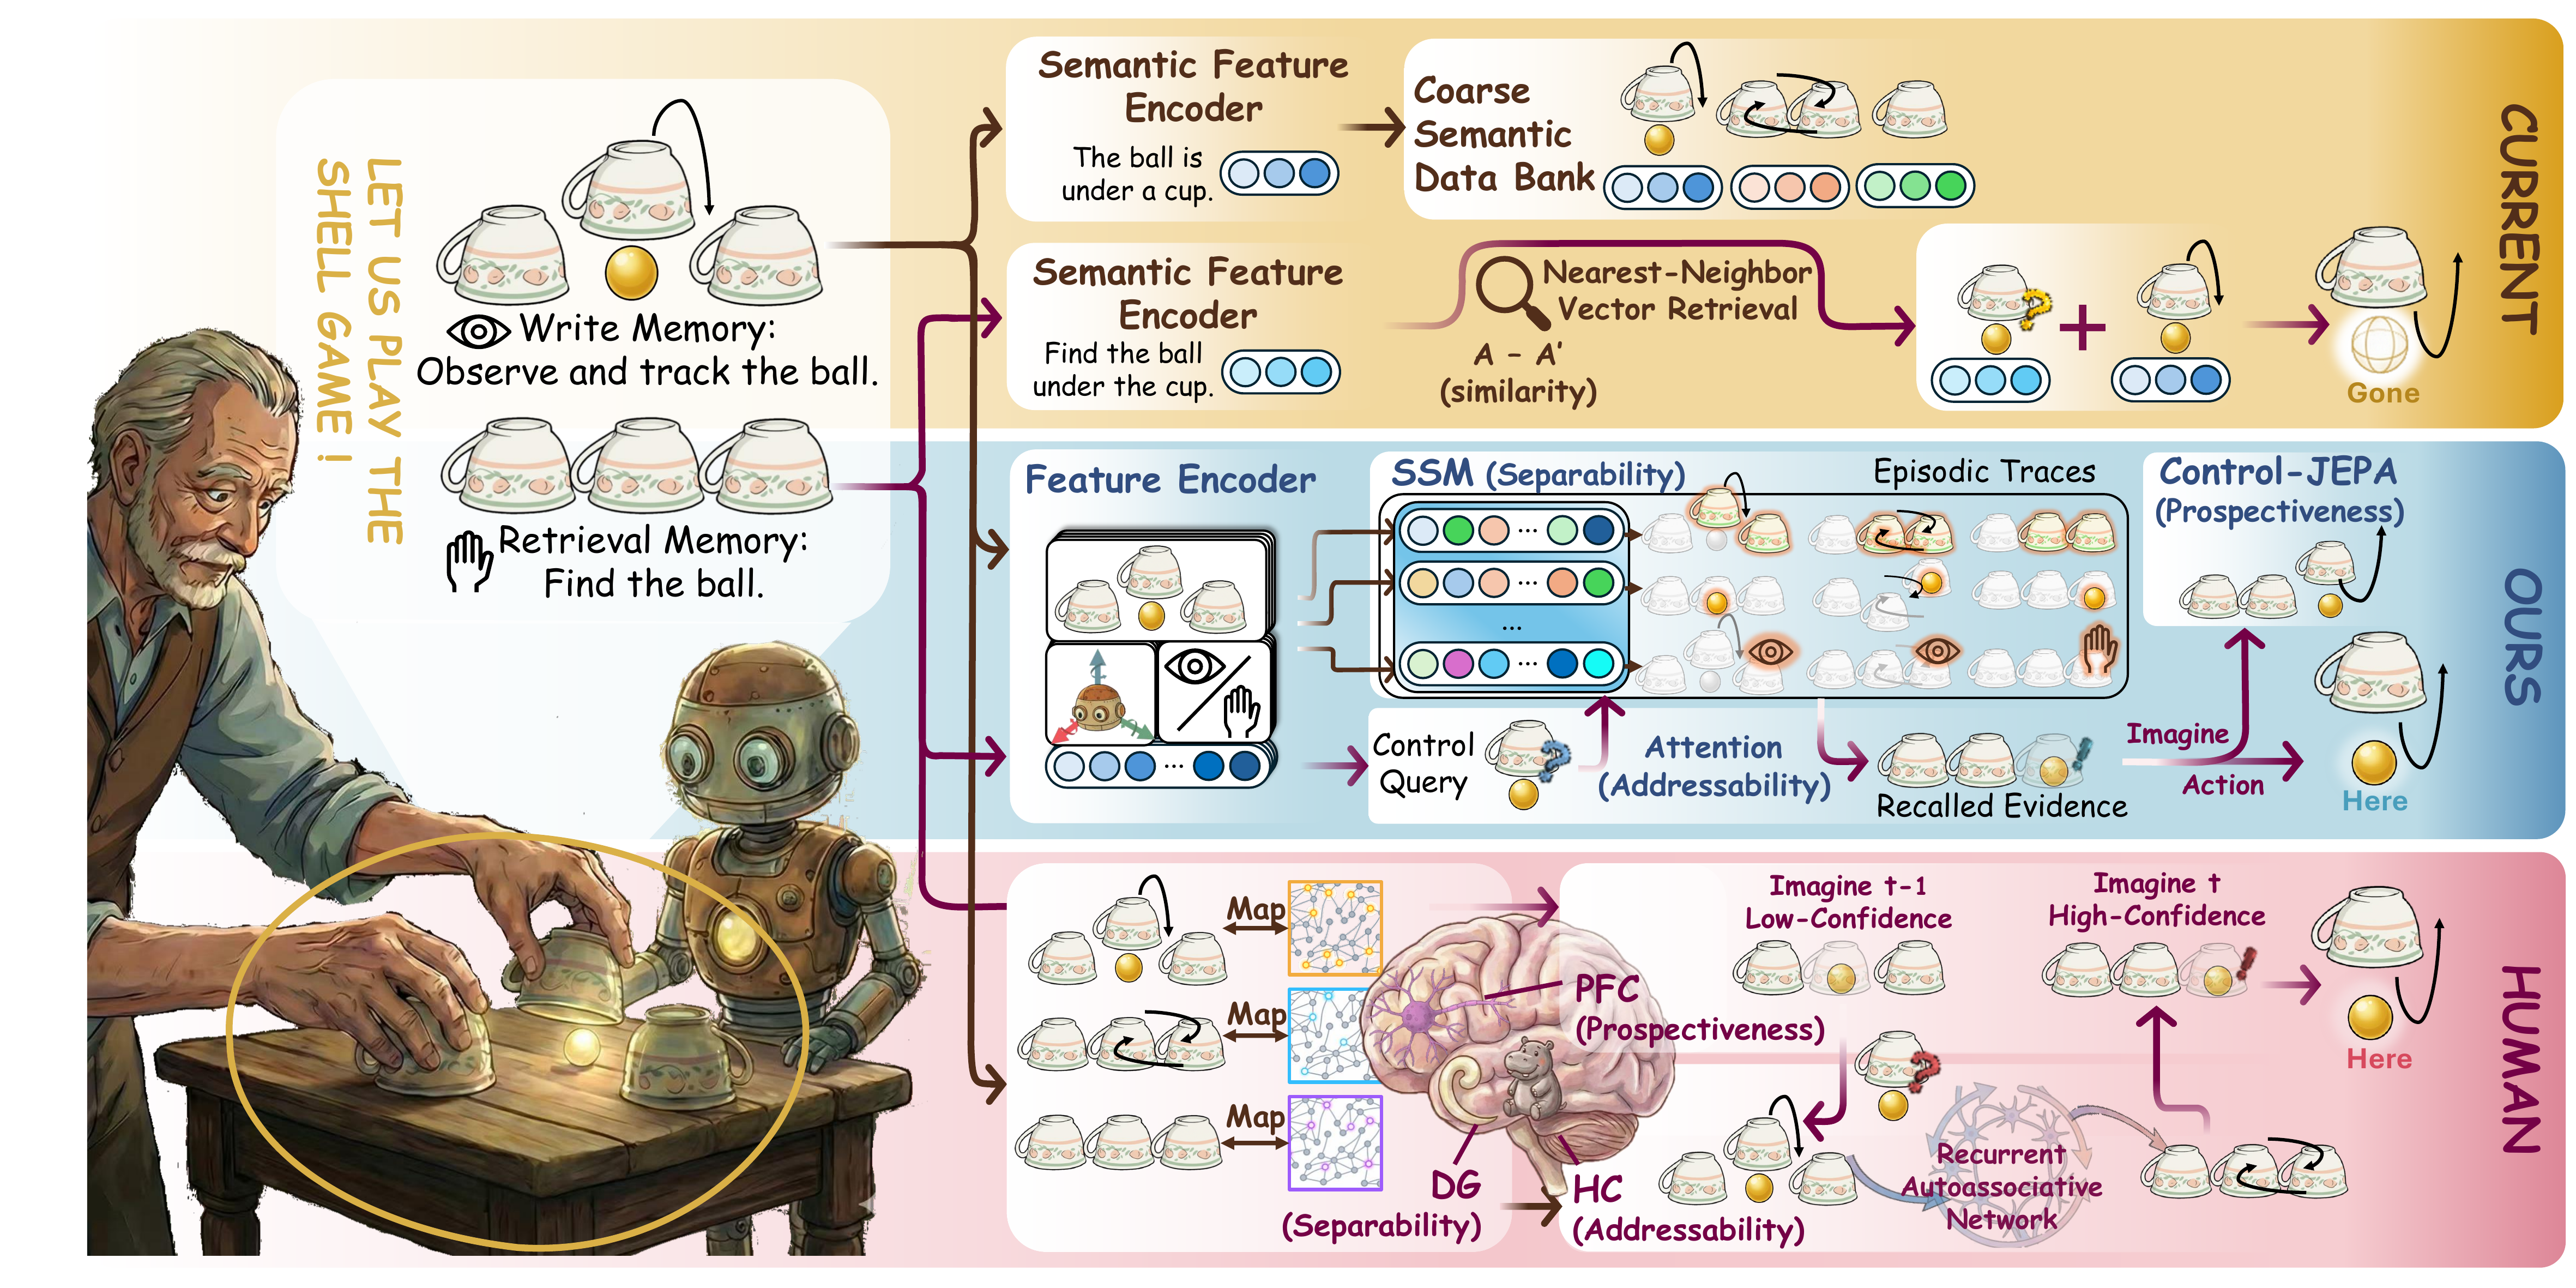
\includegraphics[width=0.96\linewidth,height=\textheight,keepaspectratio]{../../assets/figures/lecture13/ref/mem_chameleon.png}

}

\caption{观测-动作延迟需要控制索引的记忆：可区分 / 可寻址 / 可前瞻}

\end{figure}%

它主张记忆要同时满足三件事------\textbf{可区分}（不同历史要能分开）、\textbf{可寻址}（用得上时找得回）、\textbf{可前瞻}（能为将来的决策预先准备）。这三条是审视任何记忆系统的标尺，后面的工作都可以拿它来对照。

\subsection{2.4
MemoryVLA：把记忆做成显式记忆库}\label{memoryvlaux628aux8bb0ux5fc6ux505aux6210ux663eux5f0fux8bb0ux5fc6ux5e93}

如果说前面是''该有记忆''，MemoryVLA{[}7{]}
给出的是一套完整的显式记忆库。它仿照人类的双记忆系统：\textbf{工作记忆}（感知
token + 认知 token）记当下，\textbf{感知-认知记忆库}记长期历史。

\begin{figure}[H]

{\centering 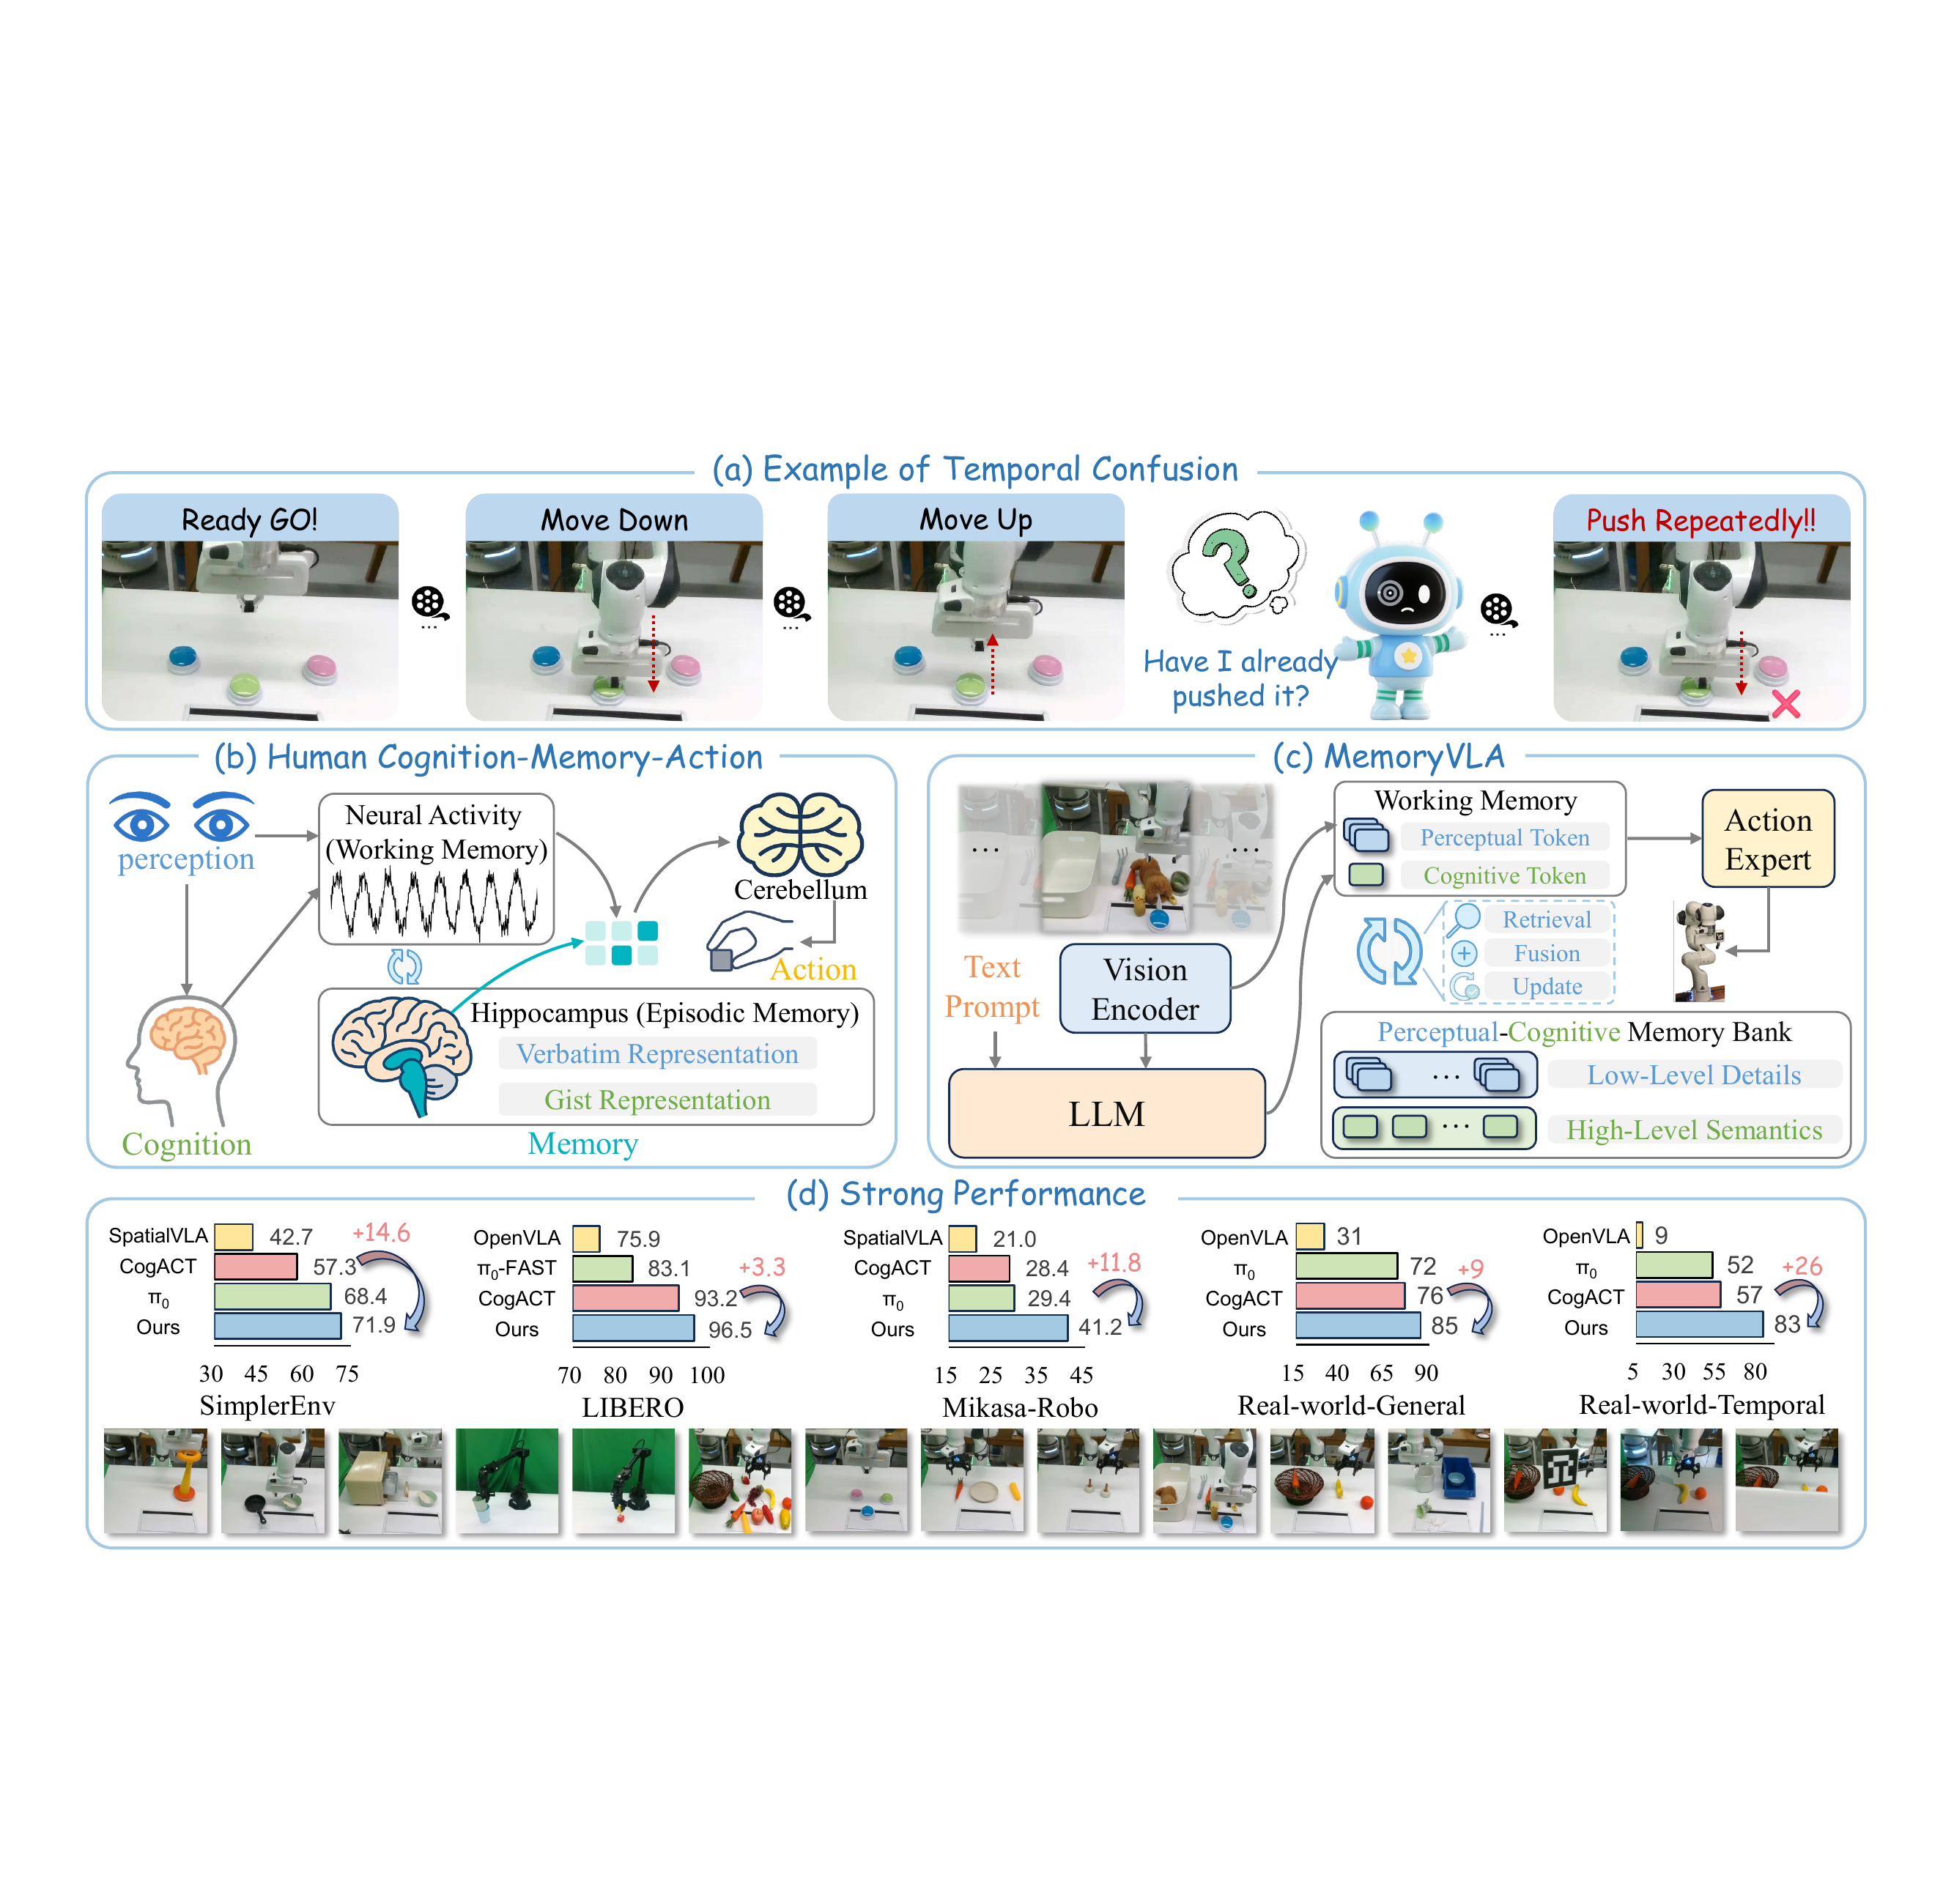
\includegraphics[width=0.94\linewidth,height=\textheight,keepaspectratio]{../../assets/figures/lecture13/ref/mem_memoryvla.png}

}

\caption{按按钮任务的非马尔可夫性、人类双记忆系统、以及感知-认知记忆库的整体设计}

\end{figure}%

三步机制：\textbf{检索}（带时间编码到记忆库里查相关历史）→
\textbf{门控融合}（自适应地把历史与当下混合）→
\textbf{巩固}（合并相邻最相似的条目，防止记忆库无限膨胀），最后由记忆条件的扩散动作专家输出动作。这套机制让它在长程真机任务上明显领先只看当下的基线。

\subsection{2.5
从''记住过去''到''预判未来''：MemoryVLA++}\label{ux4eceux8bb0ux4f4fux8fc7ux53bbux5230ux9884ux5224ux672aux6765memoryvla}

时序建模还有另一半------\textbf{想象}。按按钮任务靠记忆，传送带抓取却要靠想象（预判物体会移到哪）。

\begin{figure}[H]

{\centering 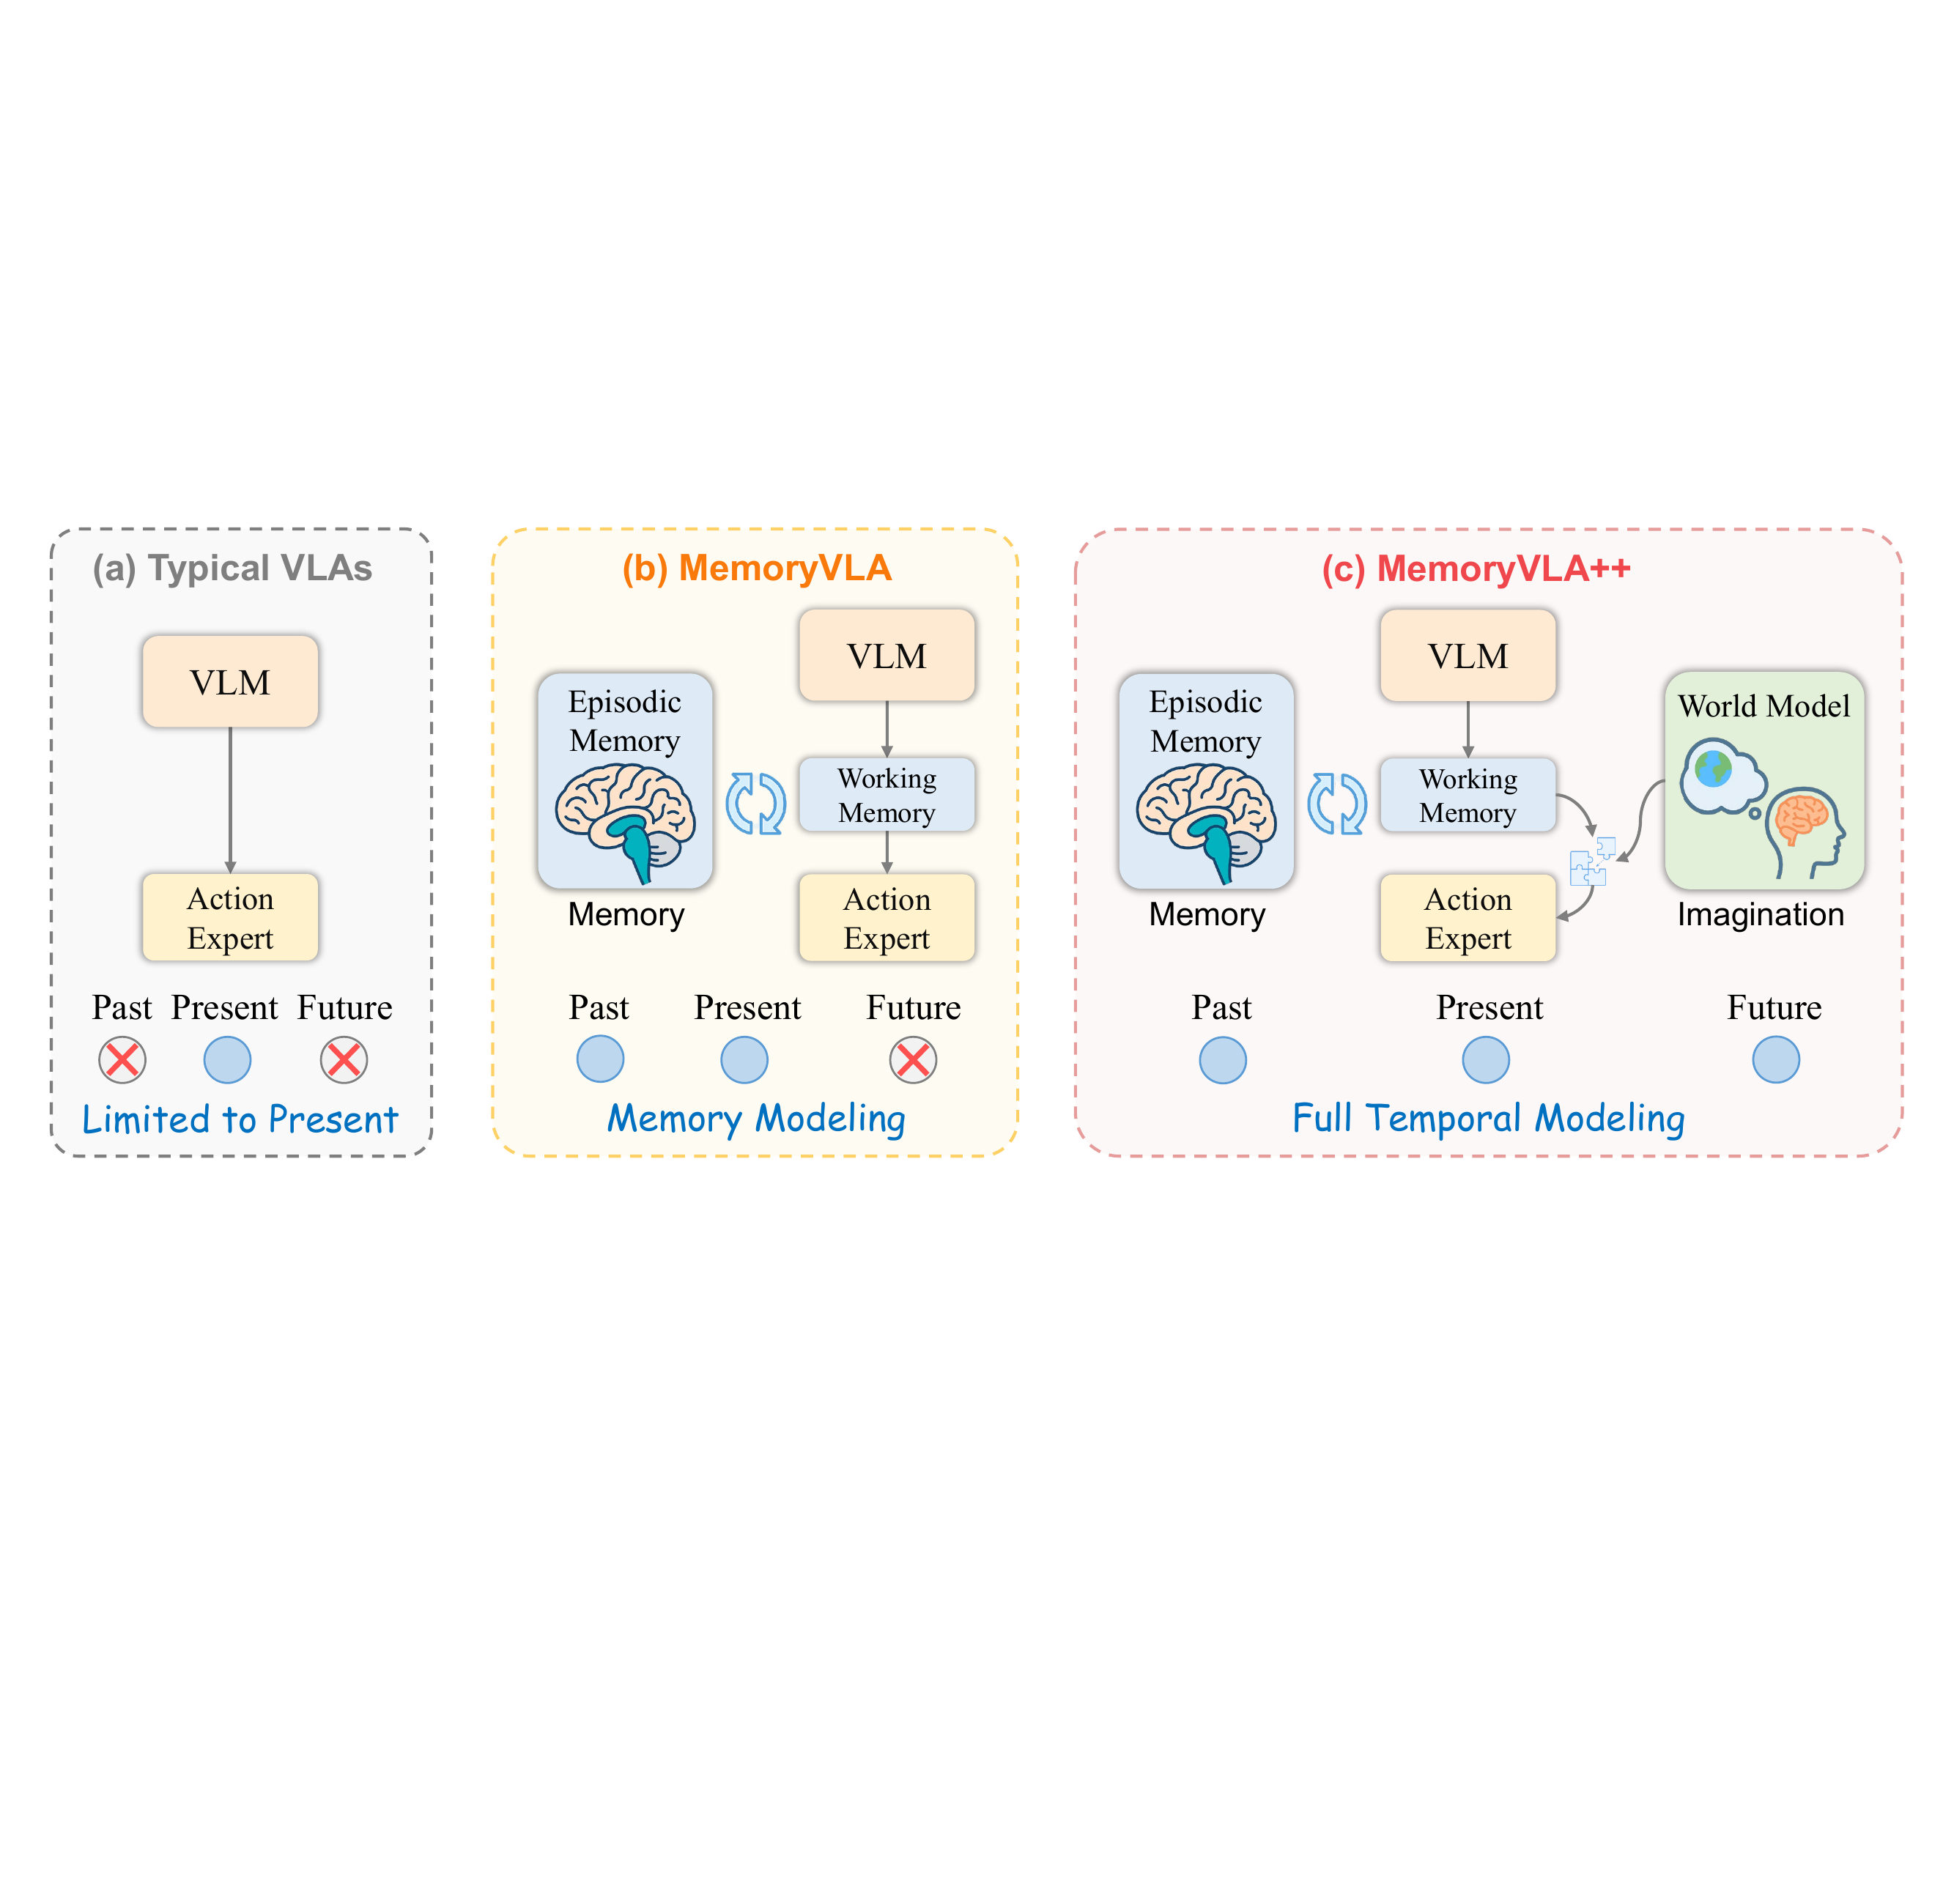
\includegraphics[width=0.86\linewidth,height=\textheight,keepaspectratio]{../../assets/figures/lecture13/ref/mem_memoryvla_pp.png}

}

\caption{三种范式：典型 VLA 只看当下 → MemoryVLA 加记忆 → MemoryVLA++
再加世界模型想象未来}

\end{figure}%

MemoryVLA++{[}8{]}
在记忆之上加一个\textbf{世界模型}，在潜空间里部分去噪出紧凑的未来
token（注意：不生成完整的像素帧，避免误差传导），让''现在 + 过去 +
未来''一起驱动动作。于是记忆与想象------时序建模的两半------终于凑齐。

\subsection{2.6
Long-VLA：把长程能力直接收口}\label{long-vlaux628aux957fux7a0bux80fdux529bux76f4ux63a5ux6536ux53e3}

无论记忆还是想象，最终都服务于\textbf{长程多步操作}。长程的难点在\textbf{技能串接}：端到端模型不擅长串接，多
policy 拼接又不统一。

\begin{figure}[H]

{\centering 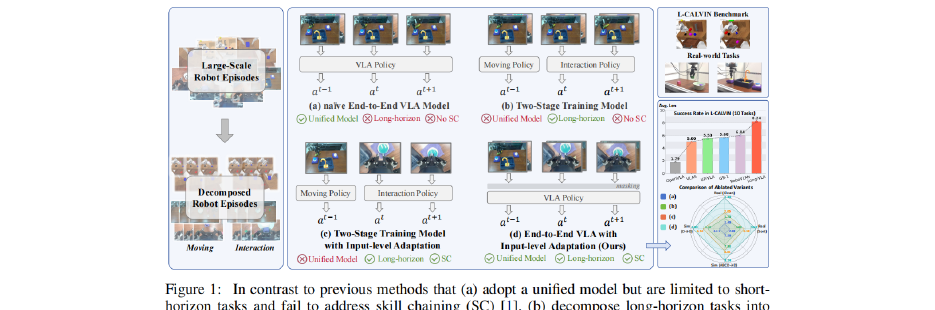
\includegraphics[width=0.96\linewidth,height=\textheight,keepaspectratio]{../../assets/figures/lecture13/ref/mem_longvla.png}

}

\caption{四种范式对比：Long-VLA 用端到端 + 输入级适配，同时做到统一 /
长程 / 会串接}

\end{figure}%

Long-VLA{[}9{]} 用 \textbf{phase-aware
输入掩码}把每个子任务切成\textbf{移动 /
交互}两段、各看各的线索，在一个端到端统一模型里拿到技能串接能力，直接以''把长任务真正做完''为目标收口。

其余几篇按这条主线各补一块：Long-Context DP{[}10{]}
把历史当隐式长上下文、用''也预测过去''逼模型用历史 +
缓存训练省成本；HAMLET{[}11{]} 给现成 VLA 外挂可学习 token +
轻记忆、免重训就变 history-aware；Dual-Memory VLA{[}12{]}
把''生成先验''和''近期动作一致性''也当记忆，让动作生成又快又稳；BagelVLA{[}13{]}
则把语言规划、视觉预测、动作生成交错进一个模型。

\subsection{2.7
易混点：三种''记忆''不是一回事}\label{ux6613ux6df7ux70b9ux4e09ux79cdux8bb0ux5fc6ux4e0dux662fux4e00ux56deux4e8b}

这条线里''记忆''和''想象''都不是单一含义，听到时要先问一句：

\begin{itemize}
\tightlist
\item
  \textbf{记的是什么}：MemoryVLA 记的是\textbf{观测历史}；HAMLET
  记的是每步压缩的 \textbf{token}；Dual-Memory 记的是\textbf{生成先验 +
  近期动作}；Long-Context DP
  根本不建记忆库，只把历史当\textbf{长上下文}。
\item
  \textbf{想象怎么做}：MemoryVLA++
  是\textbf{世界模型潜空间想象}；BagelVLA 是\textbf{语言规划 +
  视觉残差预测}。都想''看未来''，一个偏视觉生成、一个偏推理+预测。
\item
  \textbf{记忆不等于长上下文}：把历史一股脑塞进上下文只是最朴素的一种，又贵又容易错配预训练分布------这正是后面几篇要建''显式、可检索、可压缩''记忆的理由。
\end{itemize}

\subsection{2.8 本节小结}\label{ux672cux8282ux5c0fux7ed3-1}

从隐式长上下文，到显式记忆库，再到记忆 + 想象与长程收口，记忆 /
时序建模正在成为 VLA
继续往上走的关键一块拼图------它让一个只会看当下的策略，学会用过去、预判未来，把长程多步任务做成。

\section{3 人形全身
VLA：让语言驱动整个身体}\label{ux4ebaux5f62ux5168ux8eab-vlaux8ba9ux8bedux8a00ux9a71ux52a8ux6574ux4e2aux8eabux4f53}

\subsection{3.1
人形全身难在哪}\label{ux4ebaux5f62ux5168ux8eabux96beux5728ux54ea}

桌面机械臂的
VLA，主要难在''看懂场景、选对动作''。换成人形机器人，难度会突然上一个台阶：它不是一只固定在桌边的手，而是一个会移动、会转身、会蹲下、会被上肢动作牵动重心的完整身体。所以人形全身
VLA 不是简单把动作维度加大，它同时遇到四个问题：

\begin{itemize}
\tightlist
\item
  \textbf{语言要落到全身动作}：一句''走过去挥手''不是末端位姿，而是一段全身运动风格。
\item
  \textbf{视觉要决定空间关系}：椅子在左还是右、物体远还是近，会改变身体怎么走、怎么停、怎么伸手。
\item
  \textbf{高层语义和低层控制频率差太大}：VLA
  可以慢一点想，但腿和身体必须高频稳定执行。
\item
  \textbf{数据太贵}：人形全身遥操作、动捕、真机采集都比桌面操作贵得多。
\end{itemize}

这些难点最后都收敛成同一对矛盾：

\begin{quote}
一边是''懂任务、但不会走路的大脑''，一边是''会走路、但不懂任务的身体''，怎么把这两条线拼成一个端到端、会全身干活的系统？
\end{quote}

把这两端拼起来不是某一家一步到位的，而是一串工作各自推进、逐渐拼出来的。这一节按\textbf{问题的递进顺序}走一遍（注意这是叙述线索，不等于严格的时间先后------同期工作很多是并行发布的）：先证明语言能直接驱动全身，再用一个潜在接口把''高层想''和''低层动''分开，把这个双系统大脑做成开放基础模型，然后面对''没有腿''的问题，把会走稳的身体做大并露出一个干净的接口，回头再把大脑这端的动作表示和数据补上，最后用一个解耦接口把大脑和身体正式合龙。一路看下来你会发现：不管这些工作出自哪里，它们反复落到同一批想法上------快慢双系统、teacher-student
蒸馏、把动作离散成 token，以及一个夹在高低层之间的中间接口。

\subsection{3.2
LangWBC：先证明语言能直驱全身}\label{langwbcux5148ux8bc1ux660eux8bedux8a00ux80fdux76f4ux9a71ux5168ux8eab}

最早的一道题是：如果没有视觉，只有一句语言指令，能不能让人形直接做出全身动作？LangWBC{[}14{]}
没有走传统的''语言 → 参考轨迹 →
跟踪控制器''路线，而是训练一个最终部署用的 \textbf{CVAE
Student}：输入语言和本体感知，直接输出全身动作。

\begin{figure}[H]

{\centering 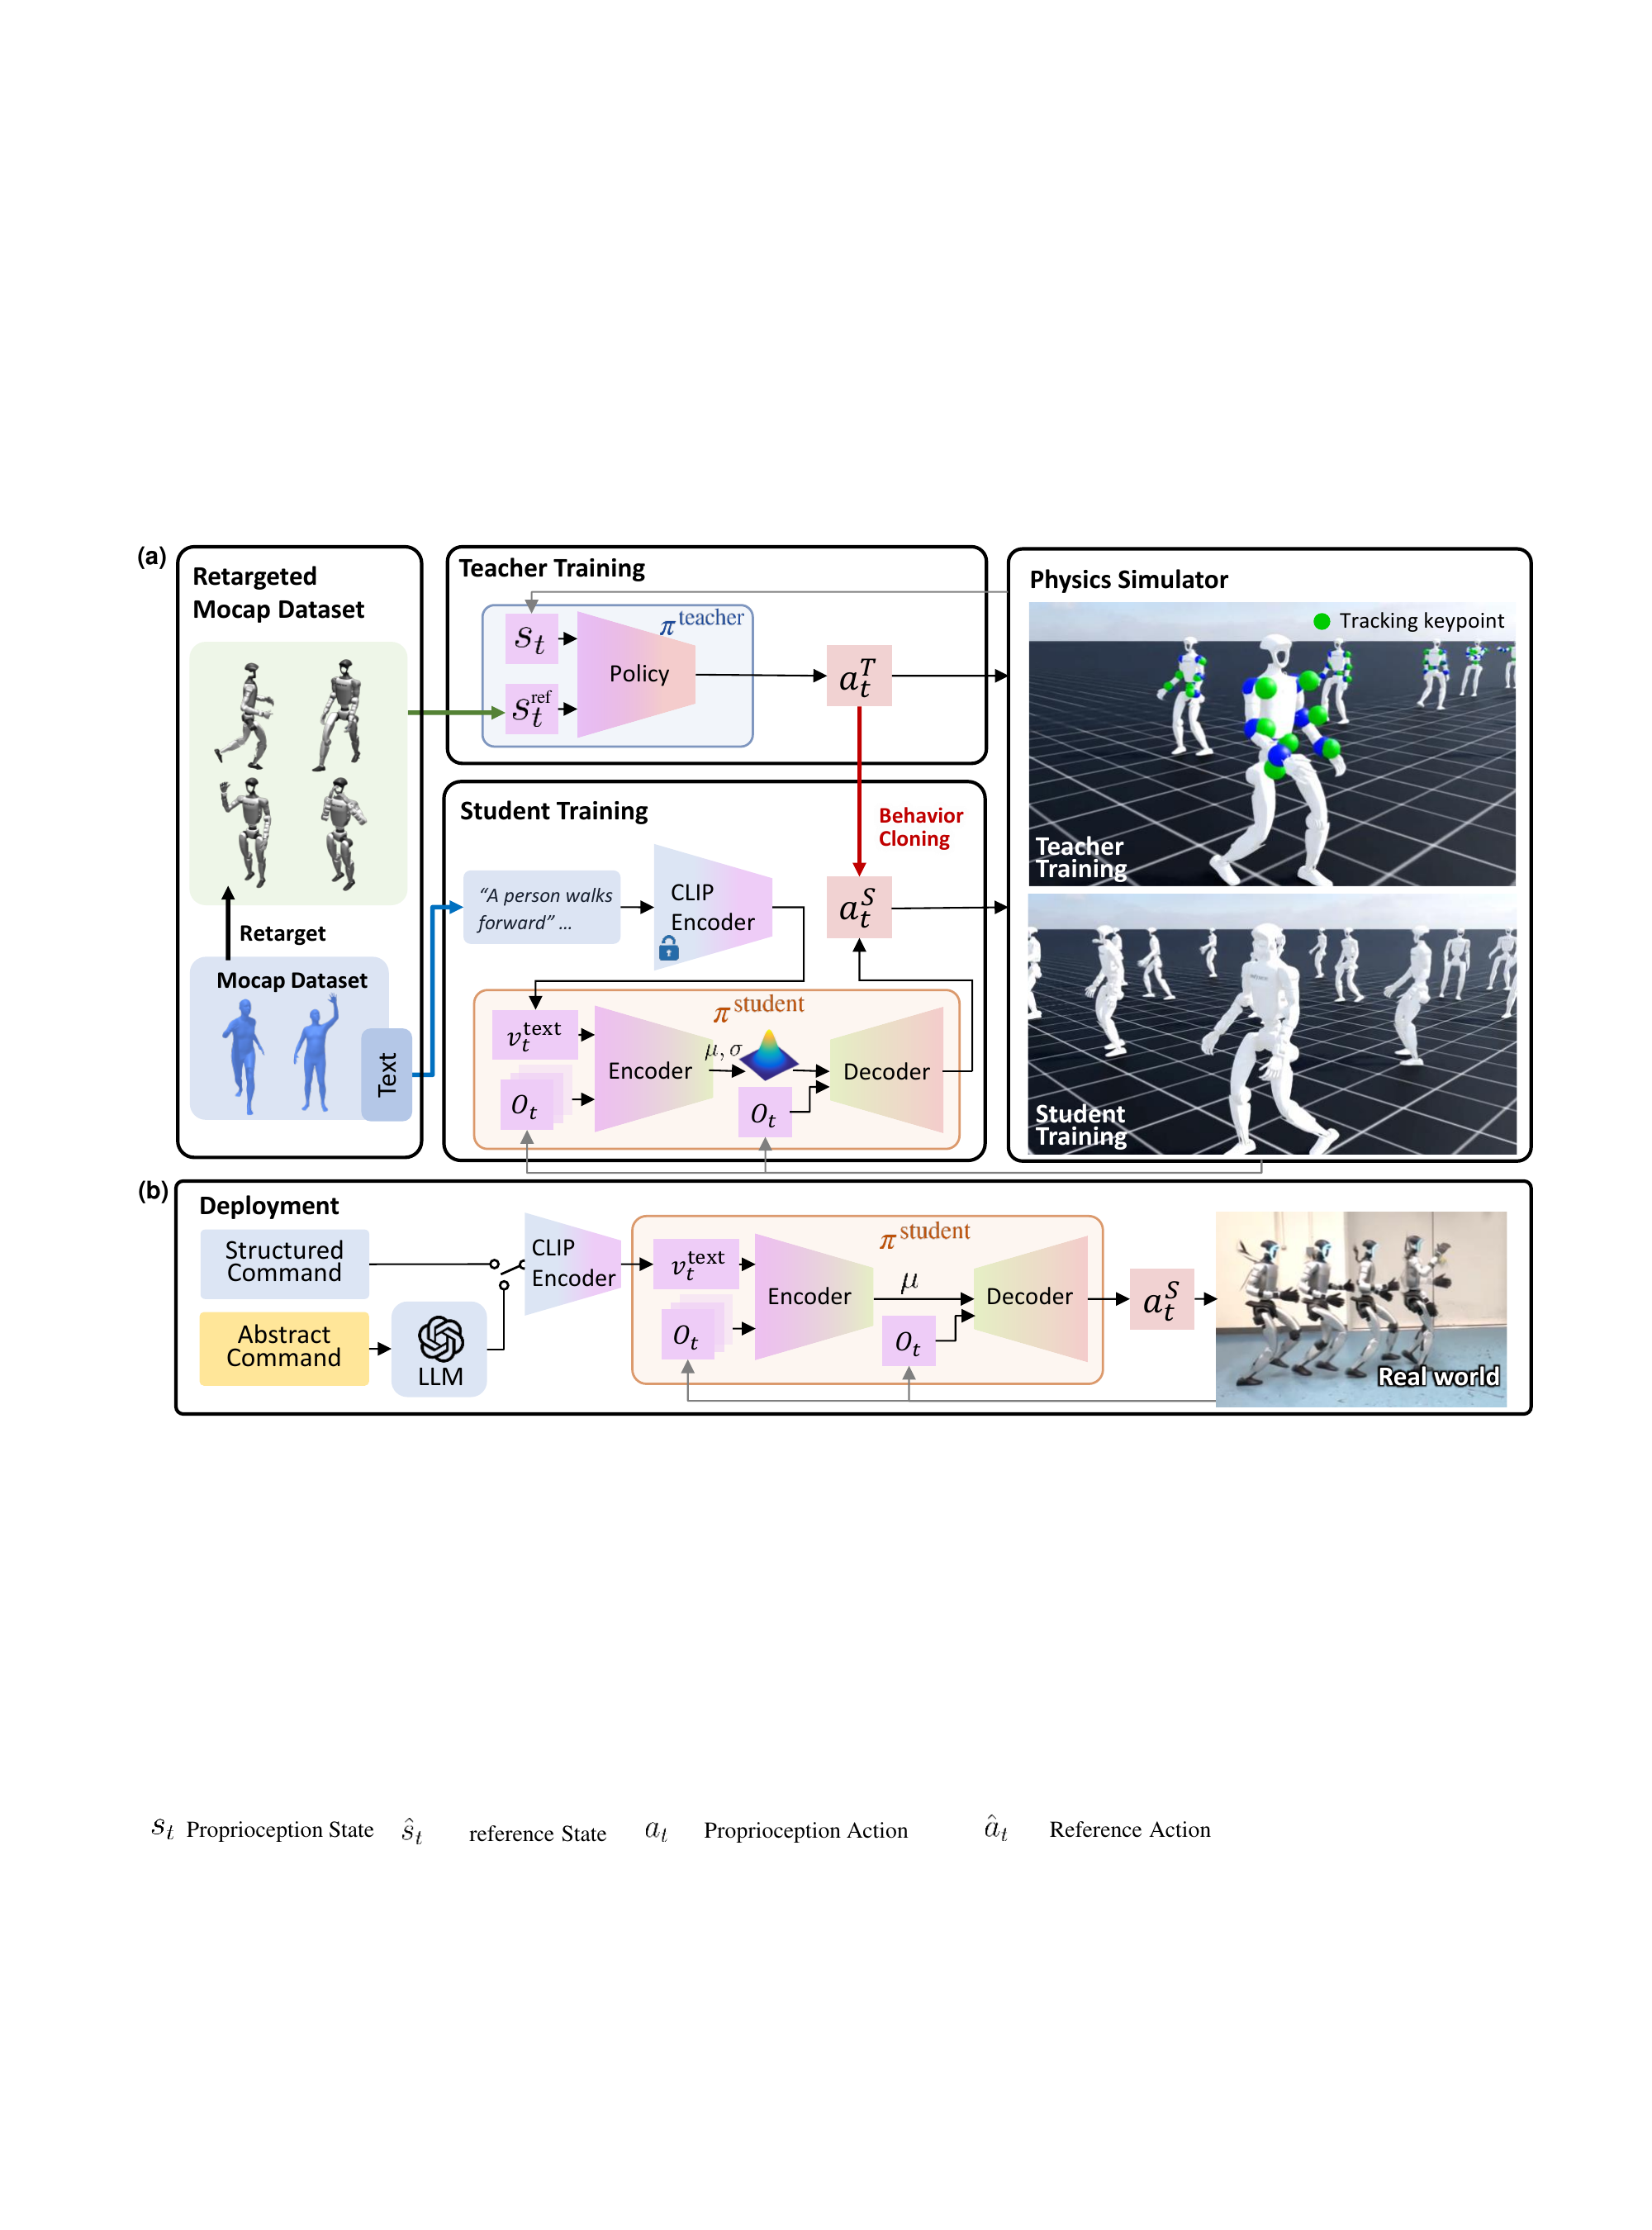
\includegraphics[width=0.88\linewidth,height=\textheight,keepaspectratio]{../../assets/figures/lecture13/ref/hum_langwbc_framework.png}

}

\caption{LangWBC 两阶段框架：先训练只会跟踪的
Teacher，再蒸馏成以语言为条件、只靠本体感知运行的 CVAE Student}

\end{figure}%

这里值得记住的是 Teacher / Student 分工：Teacher
不懂语言，只在训练中提供高质量全身动作；Student
才是部署时使用的策略，把语言条件和身体状态对齐到同一个动作空间；中间的
CVAE
隐空间像一个''动作风格旋钮''，让走、跑、挥手、转身这类动作可以泛化、切换、插值。LangWBC
先证明了一个基础能力：\textbf{语言可以直接接到人形全身控制上。}
它缺的是视觉。

\subsection{3.3
LeVERB：高层看图、低层稳执行}\label{leverbux9ad8ux5c42ux770bux56feux4f4eux5c42ux7a33ux6267ux884c}

LeVERB{[}15{]}
把视觉补了进来：机器人不只听语言，还要看第一视角图像。``坐到椅子上''这句话，椅子在哪、朝向如何，必须由视觉决定。它的核心是快
/ 慢双系统。

\begin{figure}[H]

{\centering 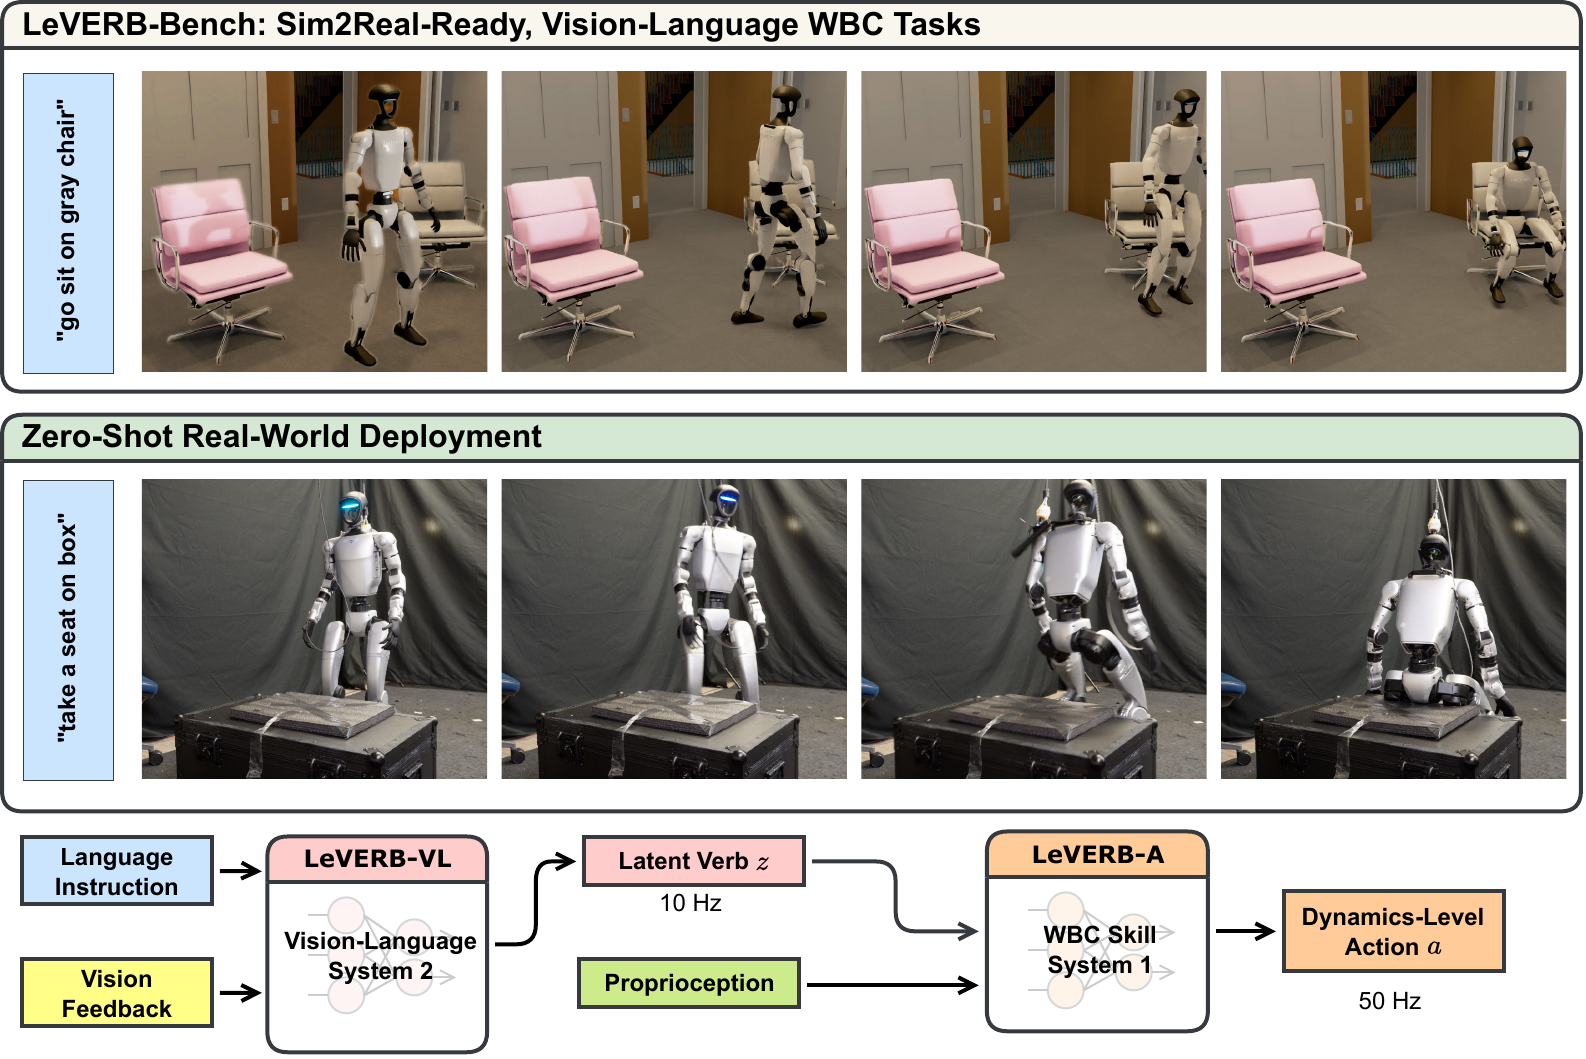
\includegraphics[width=0.86\linewidth,height=\textheight,keepaspectratio]{../../assets/figures/lecture13/ref/hum_leverb_teaser.png}

}

\caption{LeVERB 双系统：System 2 在 10 Hz 看图像和语言、输出潜在
verb；System 1 在 50 Hz 把潜在 verb 解码成全身动作}

\end{figure}%

一句话理解：\textbf{高层负责''看懂要做什么''，低层负责''把身体稳稳做出来''，中间只传一个潜在
verb。} 这个潜在 verb
不是自然语言单词，也不是关节角，而是一段动作意图的压缩表示------它就是''潜在接口''这条路线的核心范例。LeVERB
让视觉语言任务终于能接到人形全身动作上。这个''快慢双系统 +
一个潜在接口''的骨架很好用，同期也有别的工作把它推向更大规模。

\subsection{3.4 GR00T
N1：强大脑，但没有腿}\label{gr00t-n1ux5f3aux5927ux8111ux4f46ux6ca1ux6709ux817f}

GR00T N1{[}18{]} 走的是同一个快 /
慢分层思路，但要说清两者的关系：\textbf{它们是并列、独立发布的工作，不存在谁顺着谁发展}------N1
公开更早（2025-03-18），LeVERB 随后（2025-06-16）给出了 latent verb
这个接口。N1
的贡献在于把这套分层做成一个开放、可规模化的基础模型。它要对付的根本困难是：文字和图像有互联网级数据，人形机器人却没有------每条真机轨迹都要一个人实地遥操作才能产生。N1
的主张是把异构数据按''规模''和''本体专属性''组织成一座\textbf{数据金字塔}。

\begin{figure}[H]

{\centering 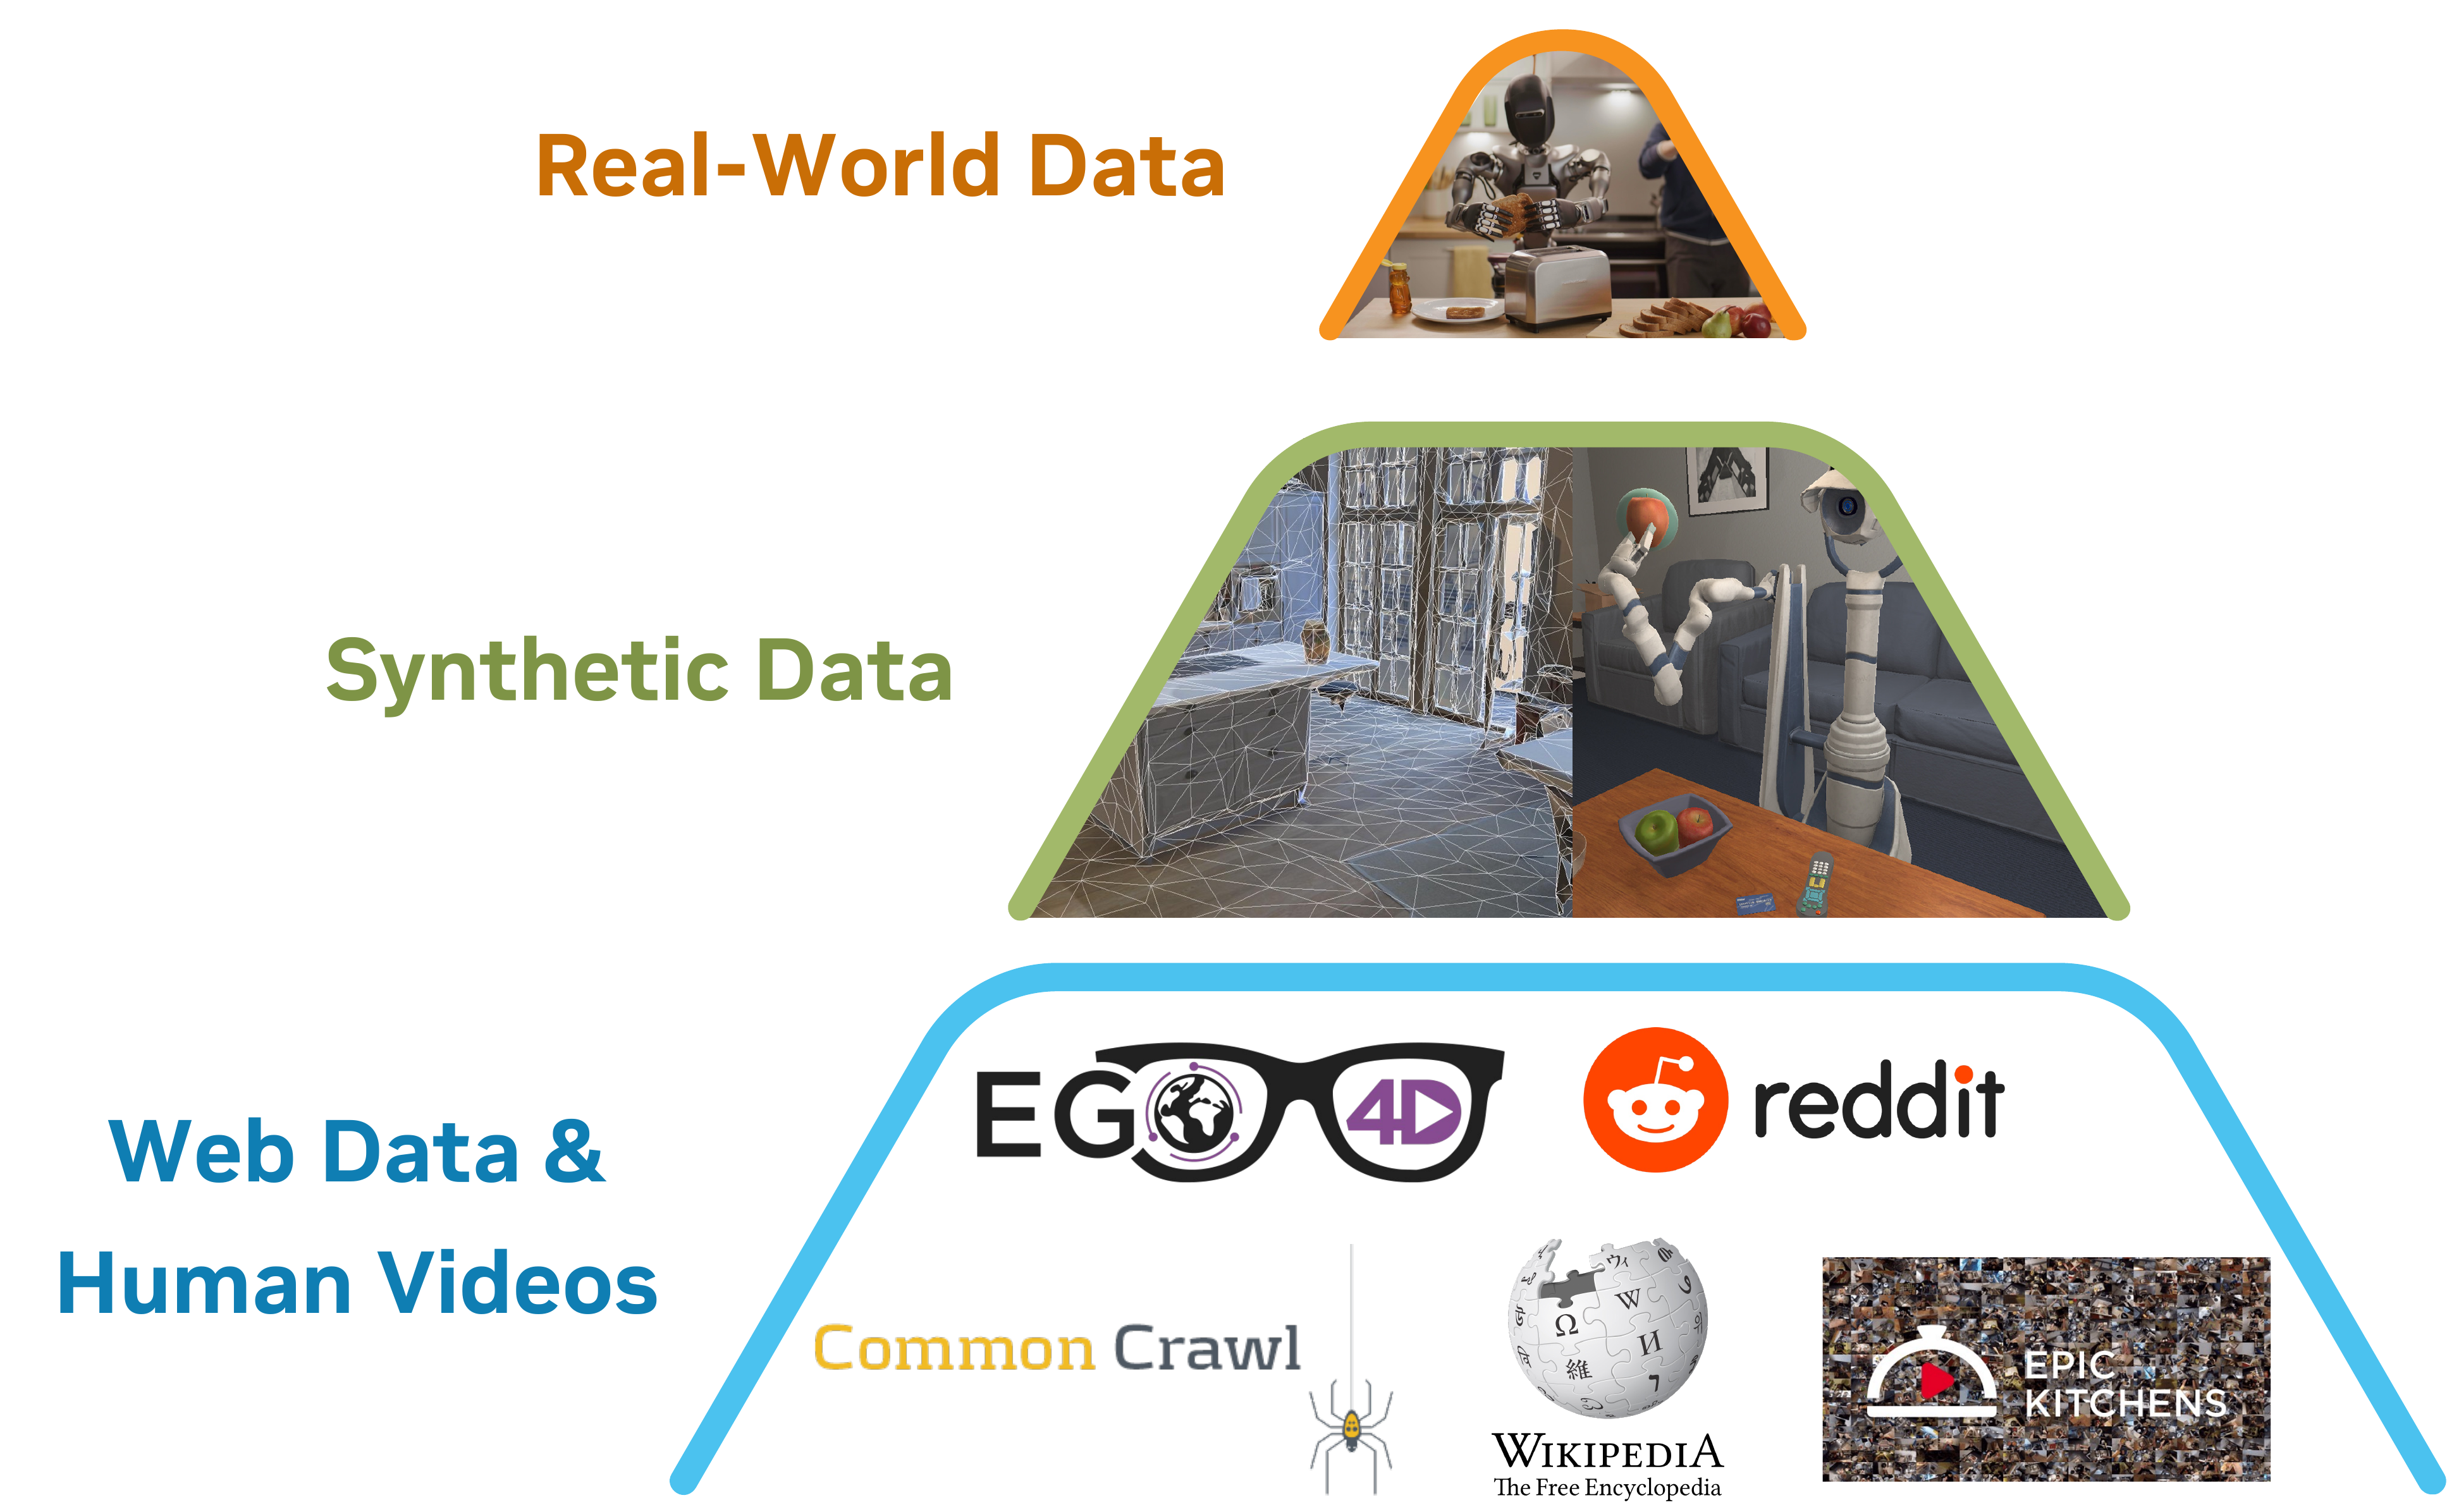
\includegraphics[width=0.56\linewidth,height=\textheight,keepaspectratio]{../../assets/figures/lecture13/ref/hum_groot_pyramid.png}

}

\caption{GR00T N1
的数据金字塔：自底向上数据量递减、本体专属性递增------底层网页与人类视频，中层仿真与合成数据，顶层真机遥操作轨迹}

\end{figure}%

模型本身就是这样一个双系统 VLA：一个作为 System 2 的 VLM
负责''想清楚要干什么''，一个作为 System 1 的 flow-matching DiT
负责''把动作流畅地动出来''，两者用交叉注意力相连------和 LeVERB
属于同一类快 / 慢分层设计，只是被做成了开放基础模型。

\begin{quote}
备注：论文里的 System 1 / System 2
是\textbf{架构分工}，示意图上标的频率不等于部署实测值。VLM
的刷新频率、动作块的生成节奏、底层控制器的执行频率是三个不同的量（口径同第11讲的
3.3.4），要各自对照论文明确报告的数字，不能用一个 Hz 概括整套系统。
\end{quote}

\begin{figure}[H]

{\centering 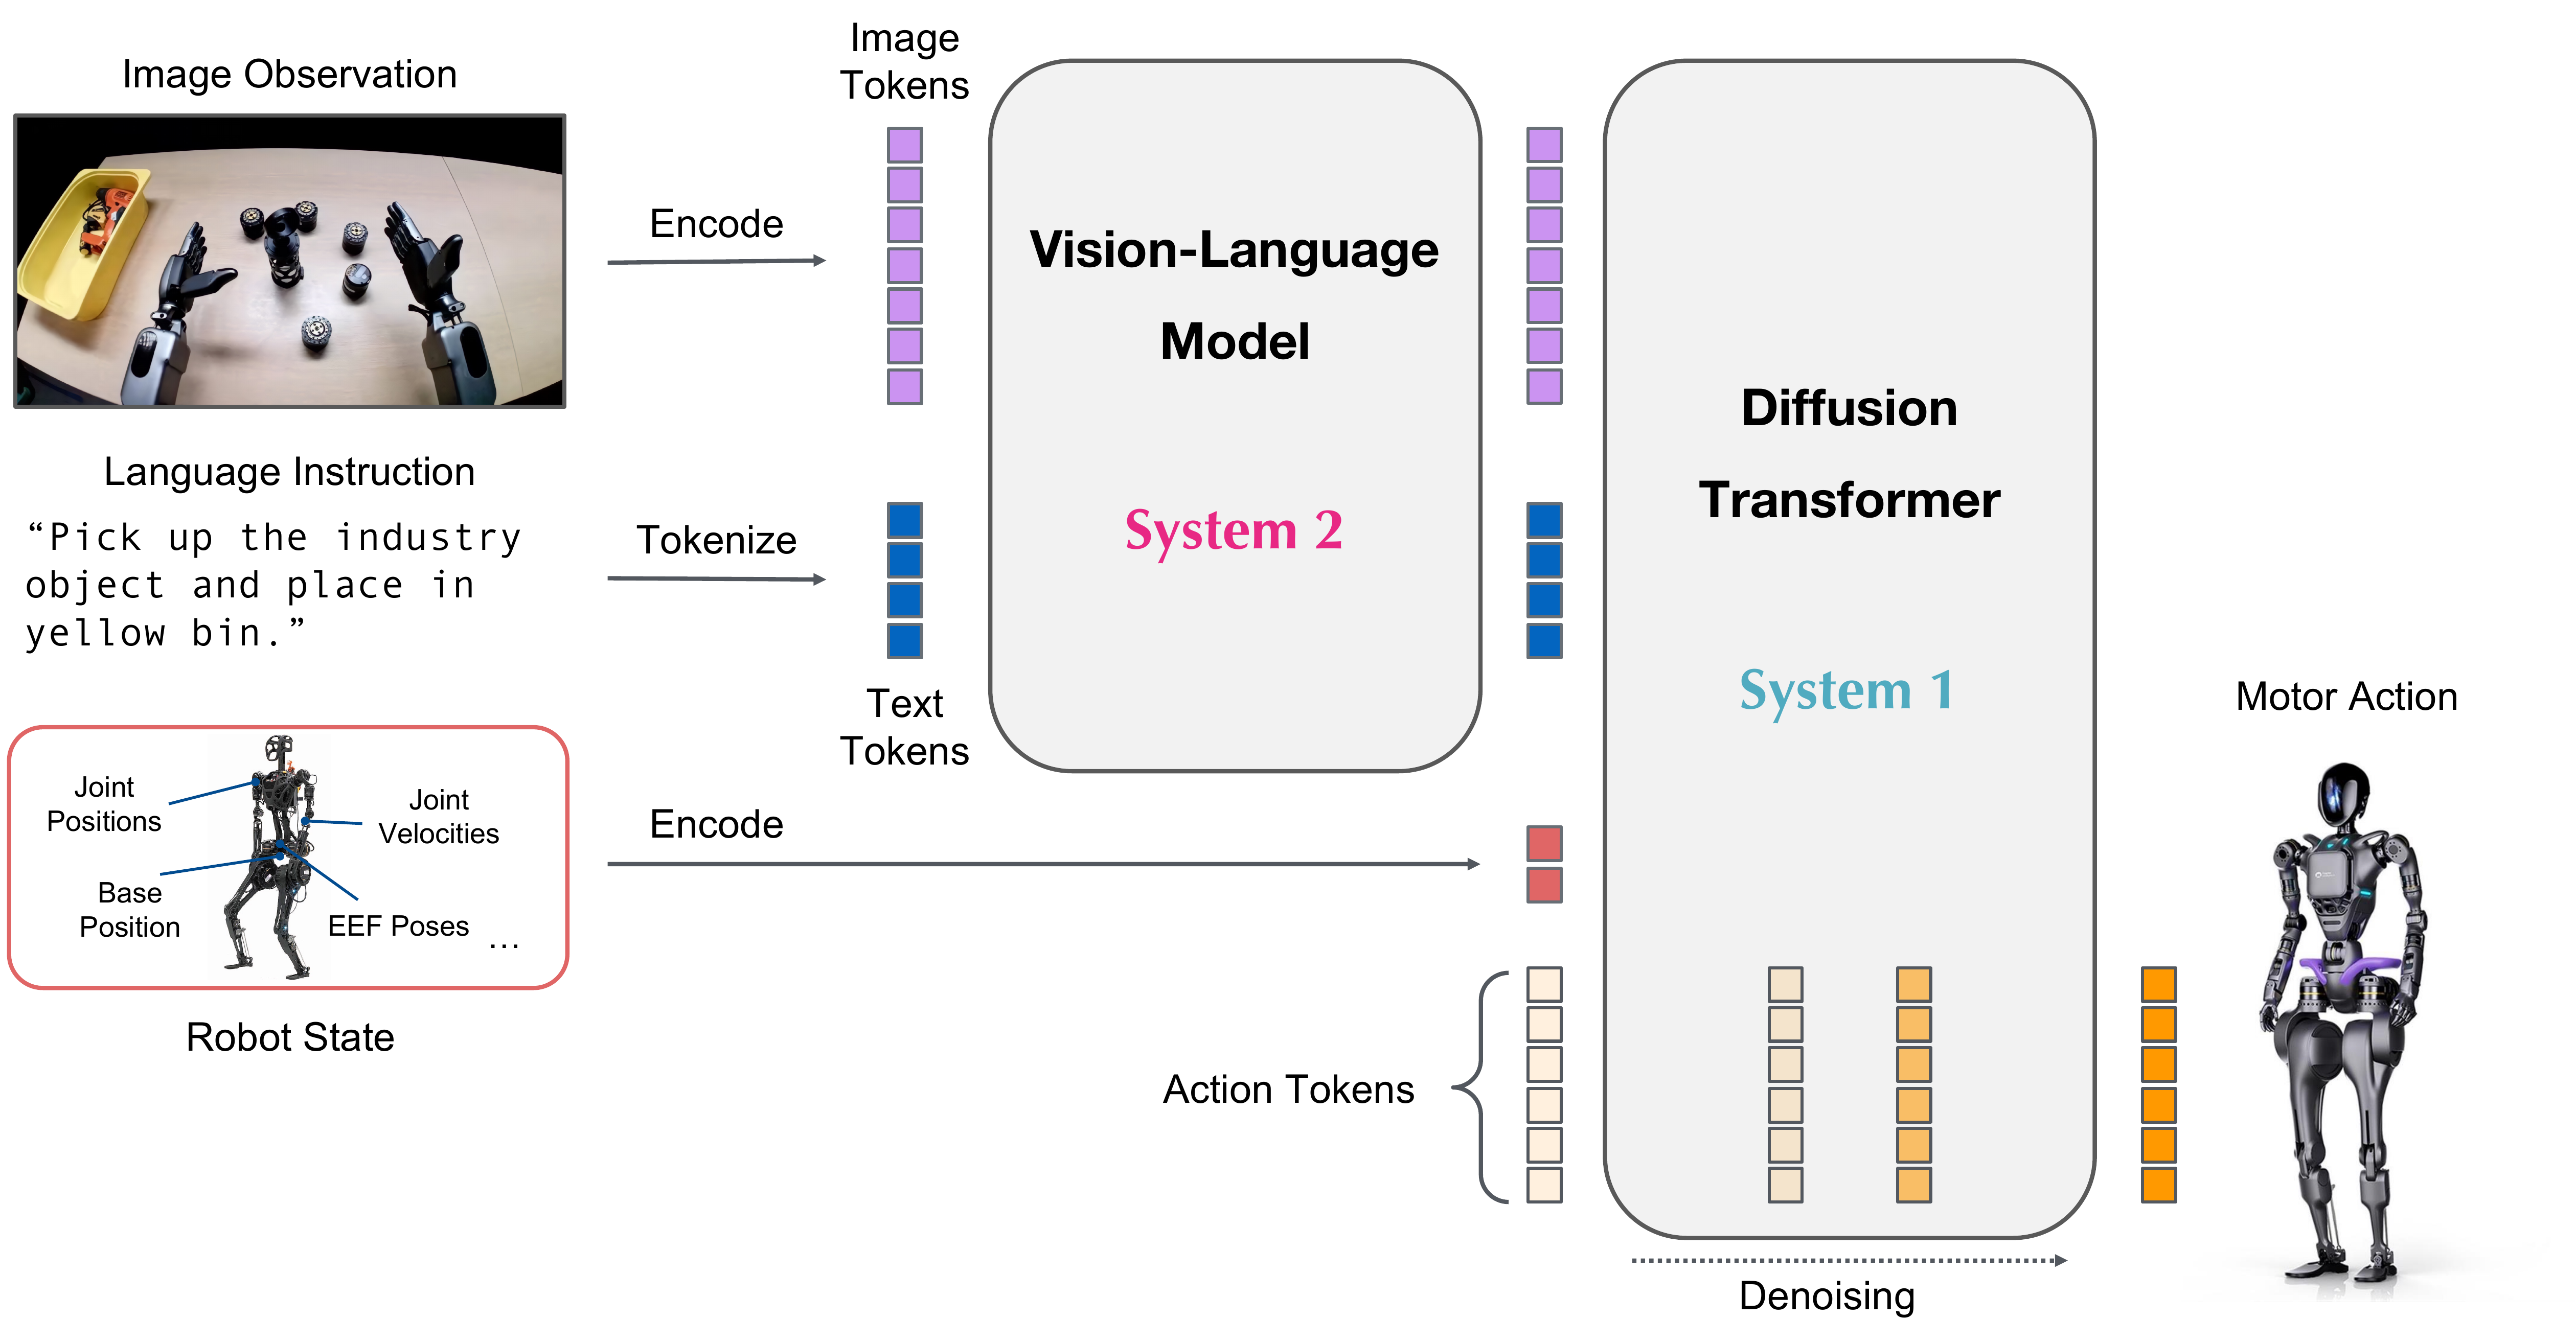
\includegraphics[width=0.8\linewidth,height=\textheight,keepaspectratio]{../../assets/figures/lecture13/ref/hum_groot_n1_inference.png}

}

\caption{GR00T N1 推理总览：图像与语言先转 token 交给 VLM，VLM
输出连同机器人状态送进 Diffusion Transformer，迭代去噪生成电机动作}

\end{figure}%

但 N1
第一版只做短时程桌面操作，论文的局限性写得很直白------\textbf{长时程的全身
loco-manipulation
还没有}。正是这个''有强大脑、却没有全身底座''的缺口，定义了下一步要补的东西：一个真正会走、会稳的身体。

\begin{quote}
备注：N1
内部确实用了潜在动作，但那是\textbf{训练期给无动作视频打伪标签的工具}，不是推理期''高层决策接全身控制器''那种分层接口。别把两者混为一谈。
\end{quote}

\subsection{3.5 HOVER：立底座}\label{hoverux7acbux5e95ux5ea7}

要补的正是这条''腿''。HOVER{[}19{]}
的洞察是：\textbf{全身运动模仿可以当所有控制模式的公共底座。}
不管最后要''走快点''还是''把手举到这里''，背后都指向同一件事------让机器人像人一样稳、协调地动。

\begin{figure}[H]

{\centering 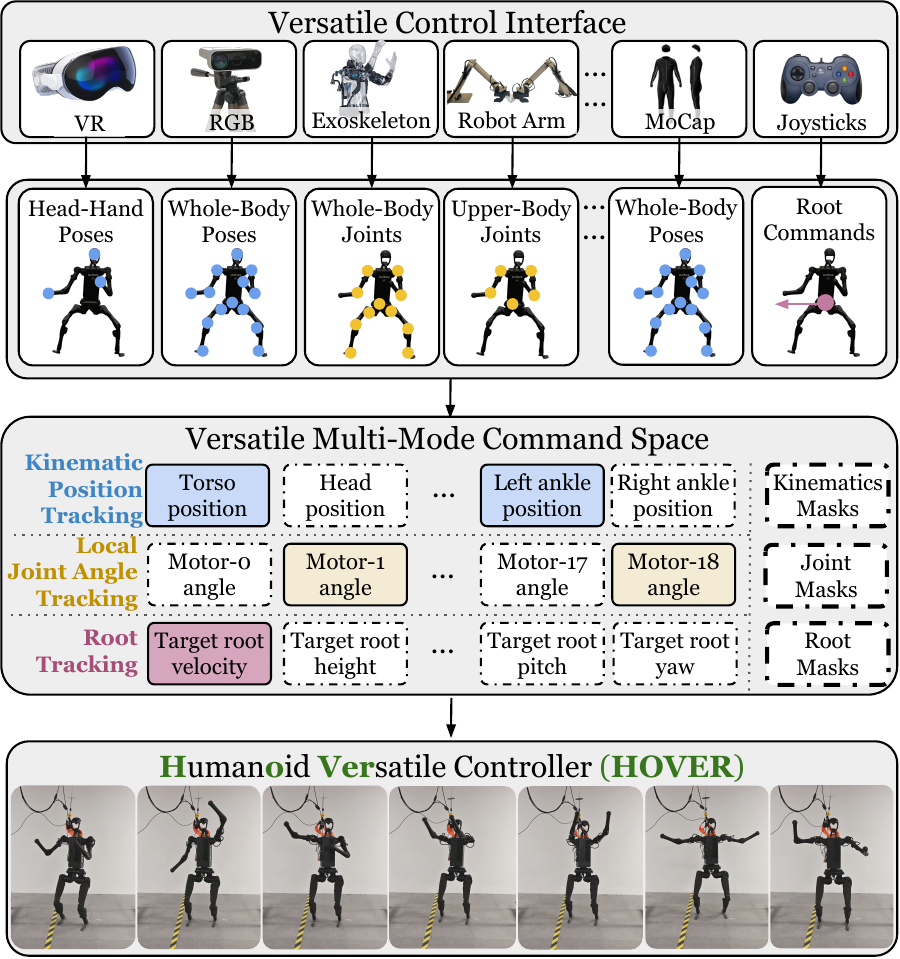
\includegraphics[width=0.9\linewidth,height=\textheight,keepaspectratio]{../../assets/figures/lecture13/ref/hum_hover_command.png}

}

\caption{HOVER 的统一命令空间：身体分上 /
下半身，每个维度用三种原子模式之一跟踪；过去每篇论文的命令空间都只是这个大空间的一个子集}

\end{figure}%

做法是先用大规模人类动捕训一个看得到完整信息的 oracle
老师，再蒸馏进一个只看得到残缺指令的学生：一张网就吃下走、跳、遥操作等十几种模式，且在多数模式上反超各自的专用控制器。上图的统一命令空间说明了为什么------身体分上
/
下半身、每个维度用三种原子模式之一跟踪，过去每篇论文各自的命令空间都只是这个大空间的一个子集。值得一提的是，这套''oracle
老师 → 残缺指令学生''的蒸馏，和前面 LangWBC 的 Teacher → CVAE Student
是同一个套路------都靠蒸馏把一个会全身动的控制器逼出来，区别只在 LangWBC
给学生加了语言条件、HOVER 追求把所有控制模式装进一张网。

\subsection{3.6 SONIC：做大底座}\label{sonicux505aux5927ux5e95ux5ea7}

HOVER 证明了底座可以统一，SONIC{[}20{]}
接着把它做大。它诊断出人形控制吃不到''规模红利''的卡点不在算法、而在任务选择，于是把\textbf{动作追踪}当成那个可规模化的基础任务（逐帧贴近动捕轨迹，监督稠密、不用设计奖励），沿网络
/ 数据 / 算力三条轴 supersize
成一个全身控制行为基础模型，并暴露出一个干净的\textbf{通用 token 接口}。

\begin{figure}[H]

{\centering 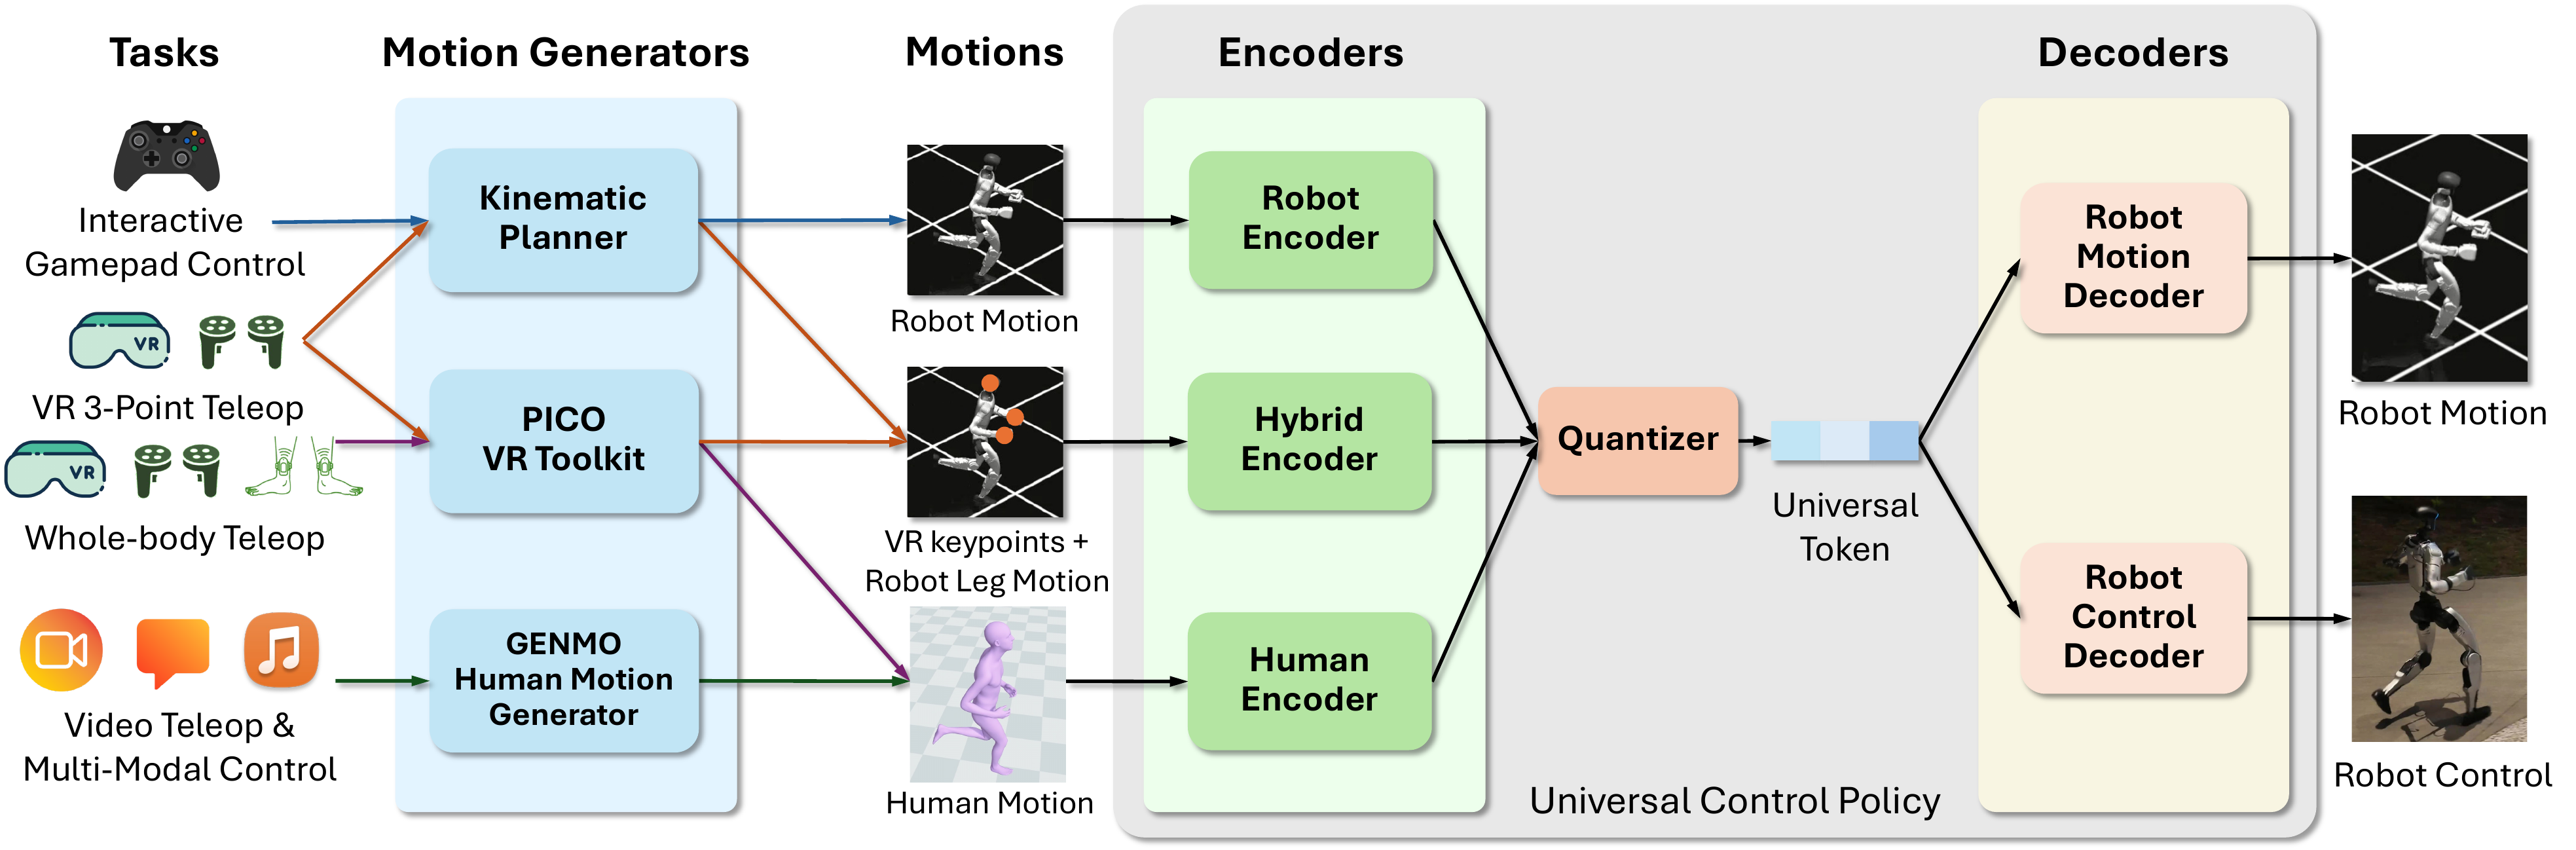
\includegraphics[width=0.9\linewidth,height=\textheight,keepaspectratio]{../../assets/figures/lecture13/ref/hum_sonic_overview.png}

}

\caption{SONIC 总览：三类指令经各自编码器进共享 latent，量化成通用
token，再由控制解码器驱动电机；同一套策略支撑手柄 / VR / 视频遥操作}

\end{figure}%

通用 token 接口最关键：现实中的指令来自手柄、VR、视频、VLA
输出，格式各异，SONIC 让它们先被翻译成同一种内部
token，再由同一个解码器变成电机命令。把这个接口接给 VLA、\textbf{让 VLA
预测 token 而不是直接预测关节角}，正是后面合龙要用的桥（见 3.9 节）。

\subsection{3.7
WholeBodyVLA：移动服务操作}\label{wholebodyvlaux79fbux52a8ux670dux52a1ux64cdux4f5c}

低层的身体和它的接口都立住了，回到大脑这端------它的能力也在同步往前补。第一块是''移动''。桌面操作默认手已经在物体旁边，可人形先得走过去------而且不是走到附近就行。WholeBodyVLA{[}16{]}
把这一步提成核心问题，叫 \textbf{manipulation-aware
locomotion}：人形不是走到某处就结束，而是要边走边为操作创造条件（走向纸袋、下蹲、侧步、抓起、搬走）。移动不再是''先导航到附近再开始操作''，而是主动把整个身体带到适合操作的位置和姿态。

\begin{figure}[H]

{\centering 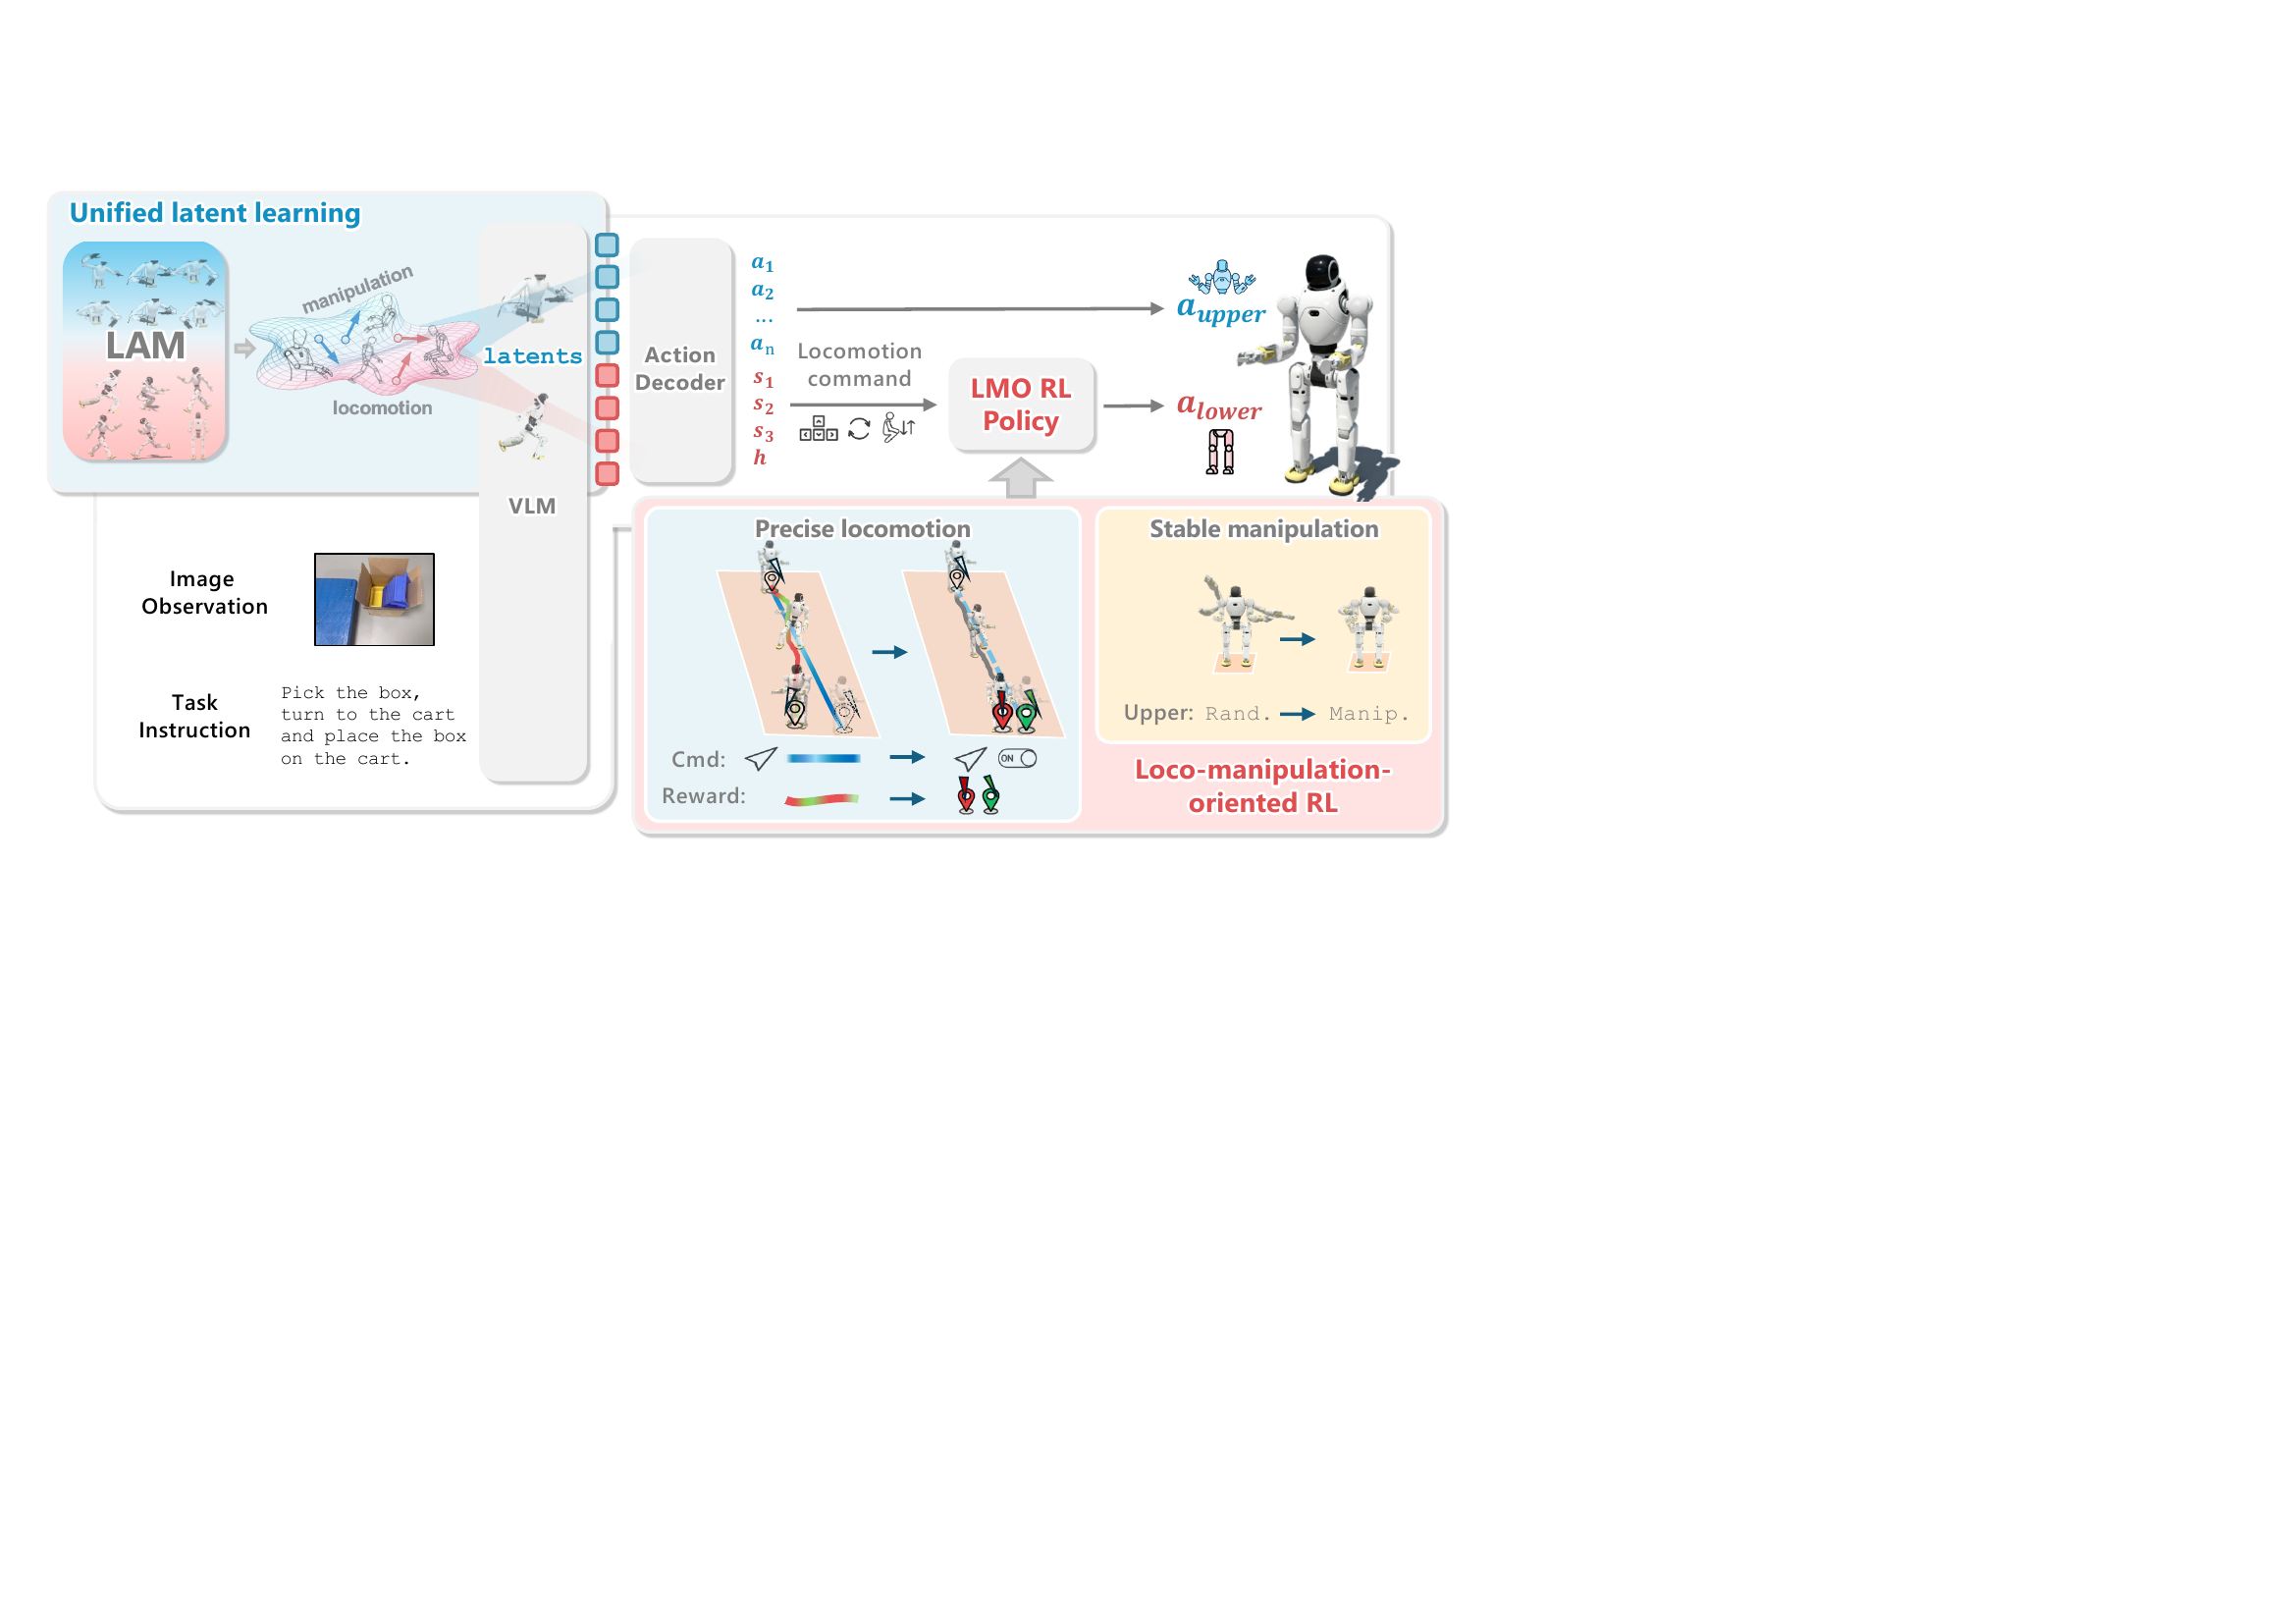
\includegraphics[width=0.92\linewidth,height=\textheight,keepaspectratio]{../../assets/figures/lecture13/ref/hum_wholebodyvla_pipeline.png}

}

\caption{WholeBodyVLA 总览：从无动作视频里学潜在动作监督，VLA
同时预测操作与移动潜在码，轻量解码器落成上肢动作和下肢指令}

\end{figure}%

实现上它从大量无动作视频里学\textbf{潜在动作}：把相邻两帧的画面变化翻译成离散伪动作标签当监督；VLA
再同时预测操作和移动两路潜在码，最后由轻量解码器分别落成上肢动作和下肢移动指令。它和前面
GR00T N1
内部''给无动作视频打伪标签''\textbf{共享同一个动机}------都想用无动作视频扩数据、绕开昂贵的真机动作标注------但技术实现并不相同：

\begin{center}
\begin{tabular}{@{}>{\raggedright\arraybackslash}p{\dimexpr 0.1385\linewidth - 2\tabcolsep\relax} >{\raggedright\arraybackslash}p{\dimexpr 0.3463\linewidth - 2\tabcolsep\relax} >{\raggedright\arraybackslash}p{\dimexpr 0.5152\linewidth - 2\tabcolsep\relax}@{}}
\toprule\noalign{}
 & GR00T N1 & WholeBodyVLA \\
\midrule\noalign{}
伪标签来源 & 在异构数据金字塔里给无动作视频打潜在动作伪标签 & 由相邻帧画面变化学出离散潜在动作码本 \\
训练目标与下游用途 & 潜在动作作为预训练监督，服务统一的双系统动作生成 & 显式预测操作 / 移动两路潜在码，再各自解码成上肢动作与下肢移动指令 \\
\bottomrule\noalign{}
\end{tabular}
\end{center}

所以别把它们读成''同一个思路''就带过去------latent
的语义和它最终被怎么用，是两者真正的分水岭。

\subsection{3.8
Humanoid-VLA：数据规模化}\label{humanoid-vlaux6570ux636eux89c4ux6a21ux5316}

第二块是''数据''。前面几篇都默认有配好的指令-动作数据可训，可人形全身数据恰恰最贵。Humanoid-VLA{[}17{]}
换到数据视角，回答''训练信号从哪来''：再漂亮的架构，没有数据也训不出来。

它的主线是''先学怎么动，再补看什么''------先把身体动作离散成
token、像语言一样做预训练（语言-运动预对齐），让模型先掌握''人形的身体怎么协调地动''；再接入第一视角视觉做条件微调，补上''看到什么、做什么''。关键一招是把海量\textbf{无标注视频}组织成自监督任务，廉价地变成可训练的指令-动作配对，绕开昂贵的真机遥操作。把身体动作离散成
motion token，和前面 SONIC 那个''通用 token''是同一个动作 token
化的思路------两边都把连续的全身动作变成一串离散
token，好让大模型像处理语言一样处理它。

\subsection{3.9 GR00T N1.5 / N1.6：用 decoupled WBC
把两条线合龙}\label{gr00t-n1.5-n1.6ux7528-decoupled-wbc-ux628aux4e24ux6761ux7ebfux5408ux9f99}

大脑这端（语言、视觉、移动、数据、动作 token）和身体那端（统一底座 +
通用 token 接口）都齐了，最后一步是把两端拼成一个端到端系统。GR00T N1.5
/ N1.6{[}21{]}
就是合龙的地方------它不是一篇新论文，而是把前面所有积木拼起来的工程节点。合龙前大脑先升级（N1.5
换更强的 VLM、加 FLARE
只对齐未来潜在表征而不生成未来画面、用合成数据扩动作；N1.6 进一步换
Cosmos-2B、把 DiT 扩到 32 层、改预测 state-relative
动作并加入更多跨本体数据）。

真正的拼法是 \textbf{decoupled WBC（解耦的全身控制）}。最朴素的想法是让
VLA
直接吐每个关节的角度，但腿的动态平衡是一套高频、对扰动极敏感的控制问题，让擅长''理解任务''的大脑同时学走路既低效又脆弱。更好的选择是：

\begin{quote}
VLA 大脑（对应双系统的
S2，慢、懂任务）只输出高层动作或目标；全身控制器（对应
S1，快、稳、会走路）接过目标，高频执行成腿 + 臂 + 手的电机命令。
\end{quote}

这正是 SONIC 那个''通用 token 接口''派上用场的地方------让大脑预测
token、底座把 token
解码成电机命令。这样两端可以独立迭代、各自规模化：大脑越做越懂任务，底座越做越稳越通用，互不拖累。绕了一圈会发现，这个解耦接口正是
LeVERB
那个''潜在接口''走到工程落地的终点------从一句话指令到全身电机命令，中间始终隔着一个干净的中间层。

\subsection{3.10 本节小结}\label{ux672cux8282ux5c0fux7ed3-2}

人形全身 VLA
的关键不是某个模型，而是一个反复出现的动作：在''想做什么''的高层语义和''怎么稳稳做出来''的低层全身控制之间，插一个潜在
/
解耦的中间接口。把它放在哪、用什么形式实现，就是这一节几篇工作的全部差别：

\begin{center}
\begin{tabular}{@{}>{\raggedright\arraybackslash}p{\dimexpr 0.3206\linewidth - 2\tabcolsep\relax} >{\raggedright\arraybackslash}p{\dimexpr 0.2701\linewidth - 2\tabcolsep\relax} >{\raggedright\arraybackslash}p{\dimexpr 0.4093\linewidth - 2\tabcolsep\relax}@{}}
\toprule\noalign{}
接口形式 & 它连接什么 & 直观作用 \\
\midrule\noalign{}
CVAE 隐变量（LangWBC） & 语言条件与动作风格 & 给全身动作留出可泛化、可插值的风格空间 \\
latent verb（LeVERB） & 视觉语言高层与 50 Hz 控制器 & 把''场景里该做什么''压成低层能执行的动作意图 \\
潜在动作（WholeBodyVLA） & 无动作视频与 VLA 训练 & 把两帧画面变化翻译成离散伪动作标签 \\
motion token（Humanoid-VLA） & 原始姿态与大模型 & 把连续身体动作变成语言模型能学习的离散序列 \\
通用 token（SONIC） & 各路指令源与同一个控制解码器 & 把手柄 / VR / 视频 / VLA 输出统一成一种内部 token \\
decoupled WBC（GR00T N1.5/N1.6） & VLA 大脑（S2）与全身控制器（S1） & 大脑只出高层目标，控制器高频执行成电机命令 \\
\bottomrule\noalign{}
\end{tabular}
\end{center}

把这张表竖着读，是同一个判断：让''想做什么''和''怎么稳稳做出来''在一个干净的接口处分工------既把复杂全身动作压进一个可沟通、可泛化的中间空间，也让大脑与身体能各自独立迭代、各自规模化。

\section{4
本讲小结与下一讲}\label{ux672cux8bb2ux5c0fux7ed3ux4e0eux4e0bux4e00ux8bb2}

\subsection{4.1
三条前沿的共同方向}\label{ux4e09ux6761ux524dux6cbfux7684ux5171ux540cux65b9ux5411}

这一讲沿三个方向看了 VLA 的前沿：实时推理（算法 + 系统 +
学习三线合力，让大模型跟上控制频率）、长时记忆（从隐式上下文到显式记忆库，再到记忆
+ 想象与长程收口）、人形全身 VLA（在高层语义和低层全身控制之间插一个潜在
/ 解耦接口，让语言驱动整个身体）。

把它们放在一起，会看到一个共同方向：\textbf{VLA
正在从''单帧、桌面、单臂''走向''高频、长程、整身''。}
快、久、全身，分别在时间的三个尺度上给 VLA
松绑------一次推理的时间、一个任务的时间跨度、一个身体的空间范围。

\subsection{4.2
下一讲：换范式进入强化学习}\label{ux4e0bux4e00ux8bb2ux6362ux8303ux5f0fux8fdbux5165ux5f3aux5316ux5b66ux4e60}

到这一讲为止，从第8讲到第13讲，我们走的都是\textbf{模仿学习}这条主线：从示教数据里学一个策略，无论是
ACT、扩散、流匹配，还是各种
VLA，本质都是''模仿专家怎么做''。它的天花板也很清楚：\textbf{纯离线的行为克隆容易受分布偏移影响}------一旦走到示教没覆盖的状态，缺少额外的纠正数据或环境反馈，恢复能力通常很有限。（这不是说模仿学习一概不会纠错：DAgger、交互式模仿、数据聚合、加入纠正与恢复数据的做法，都能把恢复行为学进来；第16讲的人在环方法就是这一路。这里说的是\textbf{没有这些补充时}的纯离线
BC。）

下一讲开始换一个范式：\textbf{强化学习}让机器人在环境里试错、用奖励塑造行为，去触碰模仿学习够不到的地方。我们会从最朴素的
REINFORCE 出发、一路升级到 PPO，让宇树 G1 先学会走路，最后再把同一套 PPO
原样搬到动作跟随上。

\section{参考资料}\label{ux53c2ux8003ux8d44ux6599}

{[}1{]} BLACK K, GALLIKER MY, LEVINE S. Real-Time Execution of Action
Chunking Flow Policies{[}EB/OL{]}. (2025-06-08){[}2026-06-26{]}.
https://arxiv.org/abs/2506.07339.

{[}2{]} LU Y, LIU Z, FAN X, et al.~FASTER: Rethinking Real-Time Flow
VLAs{[}EB/OL{]}. (2026-03-24){[}2026-06-26{]}.
https://arxiv.org/abs/2603.19199.

{[}3{]} MA Y, ZHOU Y, YANG Y, et al.~Running VLAs at Real-time
Speed{[}EB/OL{]}. (2025-10-30){[}2026-06-26{]}.
https://arxiv.org/abs/2510.26742.

{[}4{]} YANG C, HU Y, MA Y, et al.~Realtime-VLA V2: Learning to Run VLAs
Fast, Smooth, and Accurate{[}EB/OL{]}. (2026-03-31){[}2026-06-26{]}.
https://arxiv.org/abs/2603.26360.

{[}5{]} NIU J, GU K, ZHAO Y, et al.~Realtime-VLA FLASH: Speculative
Inference Framework for Diffusion-based VLAs{[}EB/OL{]}.
(2026-05-17){[}2026-06-26{]}. https://arxiv.org/abs/2605.13778.

{[}6{]} GUO X, JIANG C, KIM HB, et al.~Chameleon: Control-Indexed
Prospective Memory for Visuomotor Manipulation{[}EB/OL{]}.
(2026-03-30){[}2026-06-26{]}. https://arxiv.org/abs/2603.24576.

{[}7{]} SHI H, XIE B, LIU Y, et al.~MemoryVLA: Perceptual-Cognitive
Memory in Vision-Language-Action Models for Robotic
Manipulation{[}EB/OL{]}. (2025-08-26){[}2026-06-26{]}.
https://arxiv.org/abs/2508.19236.

{[}8{]} SHI H, LI W, XIE B, et al.~MemoryVLA++: Temporal Modeling via
Memory and Imagination in Vision-Language-Action Models{[}EB/OL{]}.
(2026-06-11){[}2026-06-26{]}. https://arxiv.org/abs/2606.09827.

{[}9{]} FAN Y, DING P, BAI S, et al.~Long-VLA: Unleashing Long-Horizon
Capability of Vision Language Action Model for Robot
Manipulation{[}EB/OL{]}. (2025-08-27){[}2026-06-26{]}.
https://arxiv.org/abs/2508.19958.

{[}10{]} TORNE M, TANG A, LIU Y, et al.~Learning Long-Context Diffusion
Policies via Past-Token Prediction{[}EB/OL{]}.
(2025-05-14){[}2026-06-26{]}. https://arxiv.org/abs/2505.09561.

{[}11{]} KOO M, CHOI D, KIM T, et al.~HAMLET: Switch your
Vision-Language-Action Model into a History-Aware Policy{[}EB/OL{]}.
(2025-10-01){[}2026-06-26{]}. https://arxiv.org/abs/2510.00695.

{[}12{]} LI Z, HU B, SHAO R, et al.~Global Prior Meets Local
Consistency: Dual-Memory Augmented Vision-Language-Action Model for
Efficient Robotic Manipulation{[}EB/OL{]}. (2026-02-25){[}2026-06-26{]}.
https://arxiv.org/abs/2602.20200.

{[}13{]} HU Y, ZHANG J, LUO Y, et al.~BagelVLA: Enhancing Long-Horizon
Manipulation via Interleaved Vision-Language-Action
Generation{[}EB/OL{]}. (2026-02-12){[}2026-06-26{]}.
https://arxiv.org/abs/2602.09849.

{[}14{]} SHAO Y, HUANG X, ZHANG B, et al.~LangWBC: Language-directed
Humanoid Whole-Body Control via End-to-end Learning{[}EB/OL{]}.
(2025-04-30){[}2026-06-26{]}. https://arxiv.org/abs/2504.21738.

{[}15{]} XUE H, HUANG X, NIU D, et al.~LeVERB: Humanoid Whole-Body
Control with Latent Vision-Language Instruction{[}EB/OL{]}.
(2025-06-16){[}2026-06-26{]}. https://arxiv.org/abs/2506.13751.

{[}16{]} JIANG H, CHEN J, BU Q, et al.~WholeBodyVLA: Towards Unified
Latent VLA for Whole-Body Loco-Manipulation Control{[}EB/OL{]}.
(2025-12-14){[}2026-06-26{]}. https://arxiv.org/abs/2512.11047.

{[}17{]} DING P, MA J, TONG X, et al.~Humanoid-VLA: Towards Universal
Humanoid Control with Visual Integration{[}EB/OL{]}.
(2025-02-20){[}2026-06-26{]}. https://arxiv.org/abs/2502.14795.

{[}18{]} NVIDIA, BJORCK J, CASTAÑEDA F, et al.~GR00T N1: An Open
Foundation Model for Generalist Humanoid Robots{[}EB/OL{]}.
(2025-03-18){[}2026-06-26{]}. https://arxiv.org/abs/2503.14734.

{[}19{]} HE T, XIAO W, LIN T, et al.~HOVER: Versatile Neural Whole-Body
Controller for Humanoid Robots{[}EB/OL{]}. (2024-10-28){[}2026-06-26{]}.
https://arxiv.org/abs/2410.21229.

{[}20{]} LUO Z, YUAN Y, WANG T, et al.~SONIC: Supersizing Motion
Tracking for Natural Humanoid Whole-Body Control{[}EB/OL{]}.
(2025-11-11){[}2026-06-26{]}. https://arxiv.org/abs/2511.07820.

{[}21{]} NVIDIA GEAR Lab. GR00T N1.5 / N1.6: humanoid whole-body control
technical report{[}EB/OL{]}. {[}2026-06-26{]}.
https://research.nvidia.com/labs/gear/gr00t-n1\_6/.




\end{document}
